\section{Auswertung}
\label{sec:Auswertung}

Zunächst wurden die Zylinder ausgemessen. Insgesamt gab es vier verschiedene Zylinder, die gegebenenfalls auch gestapelt wurden.
Die folgenden Größen wurden für die Acrylobjekte mit einer Schieblehre ermittelt:
\begin{align*}
  z_1 &= 0.0404 \unit\meter & z_2 &= 0.0615 \unit\meter \\
  z_3 &= 0.0805 \unit\meter & z_4 &= 0.1205 \unit\meter \\
  d_\text{Platte} &= 0.006 \unit\meter
\end{align*}

\subsection{Schallgeschwindigkeit und Wellenlänge mittels des Impuls-Echo-Verfahren}

Die Schallgeschwindigkeit wird über die Formel \autoref{tbd} ermittelt.
Dafür wird diese folgendermaßen umgestellt:
\begin{equation}\label{eq:c_schall}
  c_\text{Acryl} = \frac{2}{t} \cdot d_\text{Platte}
\end{equation}
Abgelesen werden die Intervalle aus \autoref{fig:messung1}, woraus sich der Mittelwert
\begin{equation}
  \increment t = 4.4 \pm 0.4
\end{equation}
und daraus wiederum
\begin{equation}
  c_\text{Acryl} = (2740 \pm 270) \cdot 10^3 \unit{\meter / \second}
\end{equation}
bildet. 

\begin{figure} [H]
  \centering
  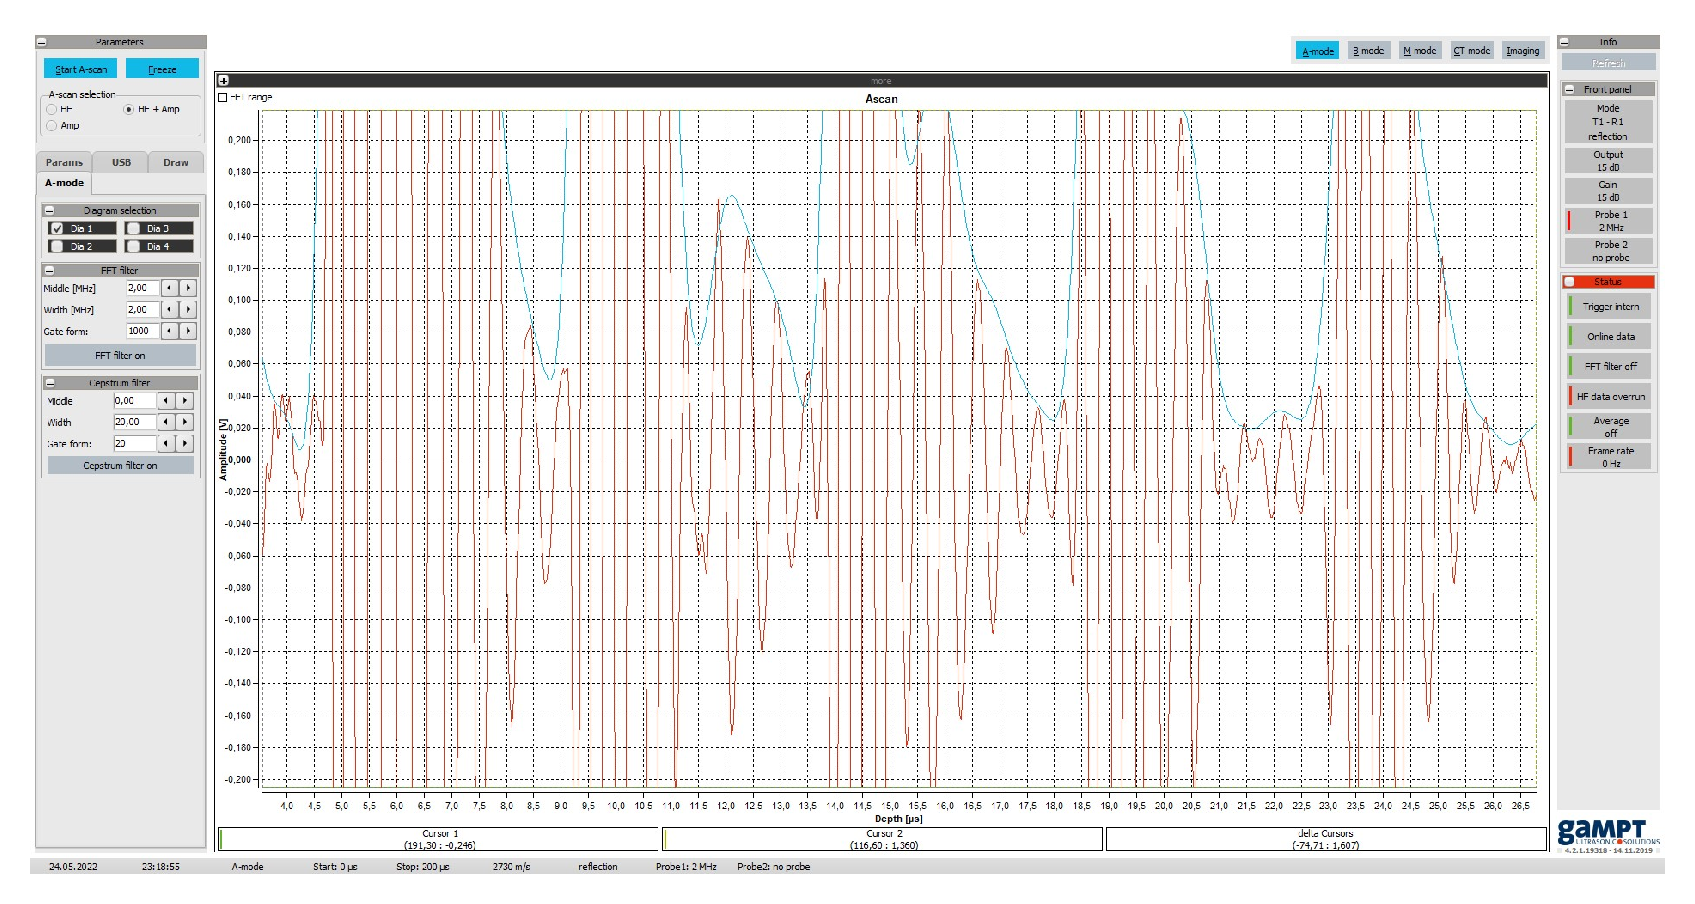
\includegraphics[width =\linewidth]{pictures/Schallgeschwindigkeit/Messung1.pdf}
  \caption{Screenshot der Messung der Acrylplatte.}
  \label{fig:messung1}
\end{figure}

Weiterhin soll die Frequenz bestimmt werden.
Dies geschieht über das Abschätzen der Periodenlänge.
Dafür werden 5 Periodenlängen aus \autoref{fig:messung2} abgelesen und gemittelt.
Daraus ergibt sich dann
\begin{equation*}
  \increment T = \frac{2.3 \, \unit{\micro\second}}{5} = 0.46 \, \unit{\micro\second},
\end{equation*}
woraus sich direkt
\begin{align*}
  f = \frac{1}{T} = 2.174 \, \unit{\mega\hertz} && \text{und} && \lambda = \frac{c}{f} = (1.26 \pm 0.12) \cdot 10^3 \, \unit\meter\\
\end{align*}
ergeben.
Die Tiefenmessung des Programms ergibt dann eine Tiefe von $d = 0.6 \, \unit{\centi\meter}$.


\begin{figure} [H]
  \centering
  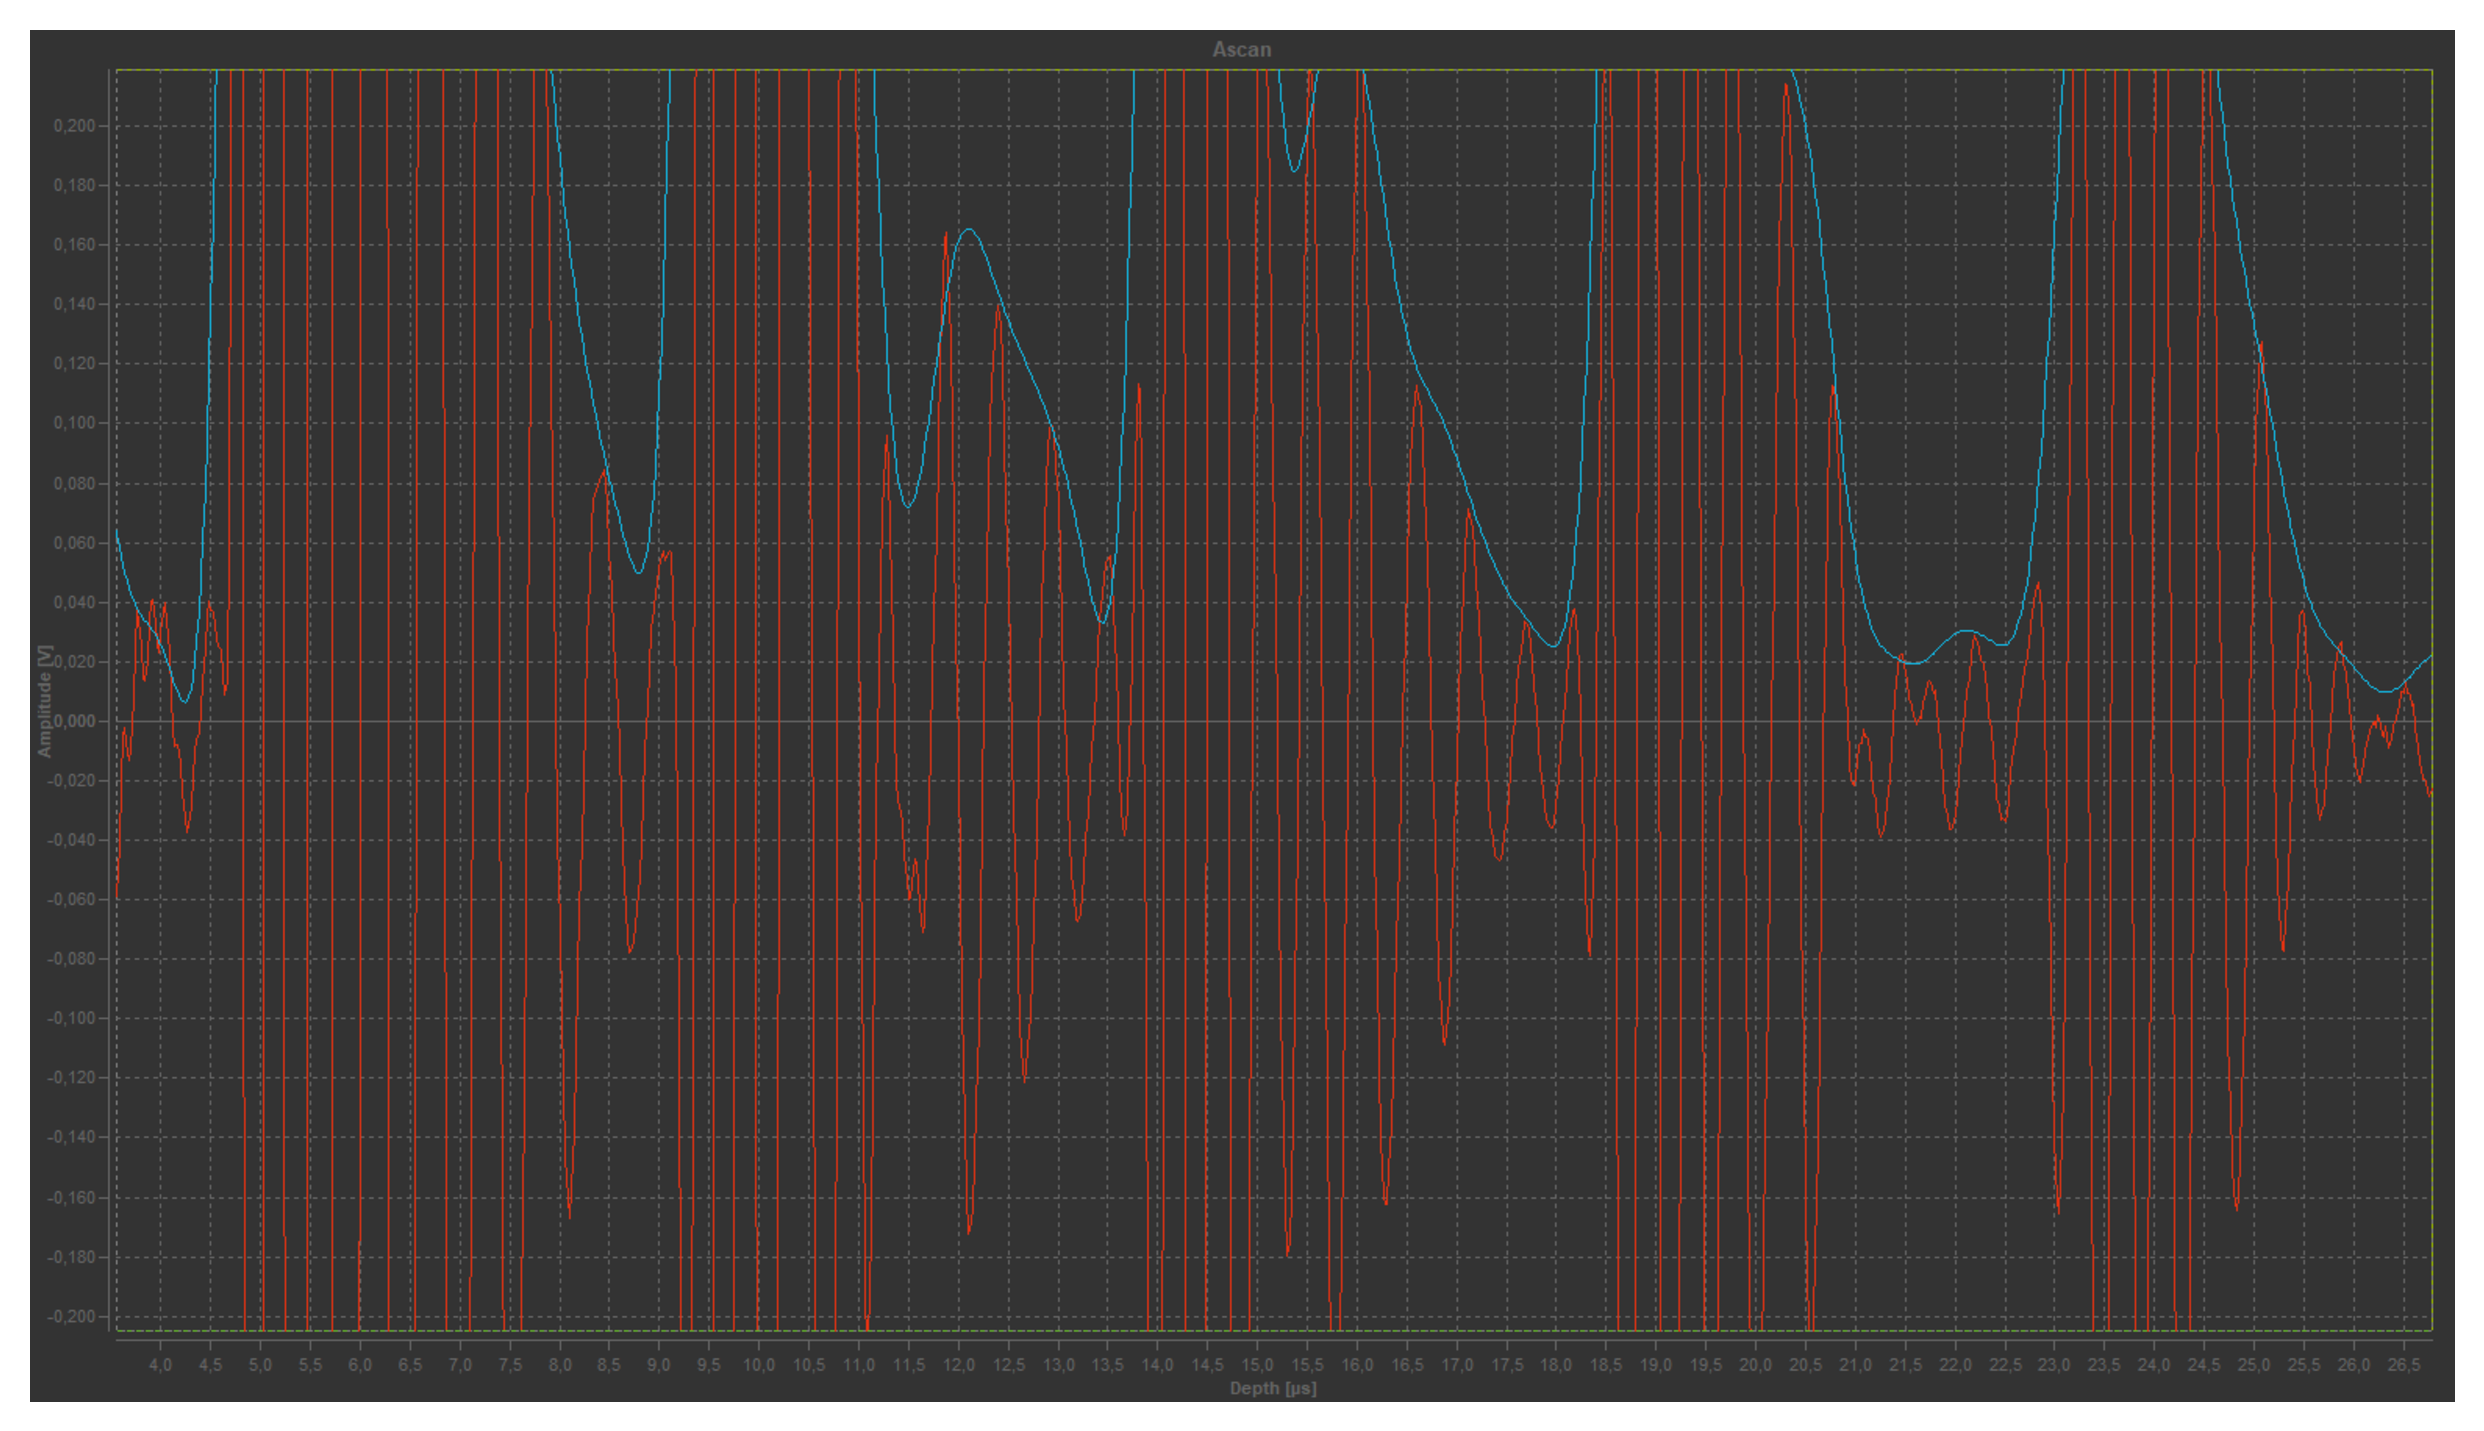
\includegraphics[width =\linewidth]{pictures/Schallgeschwindigkeit/Messung2.pdf}
  \caption{Screenshot der Messung der Acrylplatte im anderen Modus.}
  \label{fig:messung2}
\end{figure}


\subsection{Schallgeschwindigkeitsmessung mittels des Impuls-Echo-verfahrens}

Die Messungen sind in \autoref{fig:echo_messungen} zu finden.
Die daraus entnommenen Messdaten sind in \autoref{tab:echo_messungen} zu finden.

\begin{table}
  \centering
  \caption{Messdaten de3s Impuls-Echo-Verfahrens.}
  \label{tab:echo_messungen}
  \begin{tabular}{c | c c}
      \toprule
      Zylinder& Höhe / $\unit\meter$ & t / \unit{\micro\second}\\ 
      \midrule
      1     & 0.0404 & 30.3 \\
      2     & 0.0615 & 46.0 \\
      3     & 0.0805 & 59.5 \\
      1 + 2 & 0.1019 & 75.5 \\
      1 + 3 & 0.1209 &  -   \\
      4     & 0.1205 & 88.8 \\
      \bottomrule
  \end{tabular}
\end{table}



\begin{figure}%
  \begin{subfigure}{0.48\textwidth}%
  \centering%
  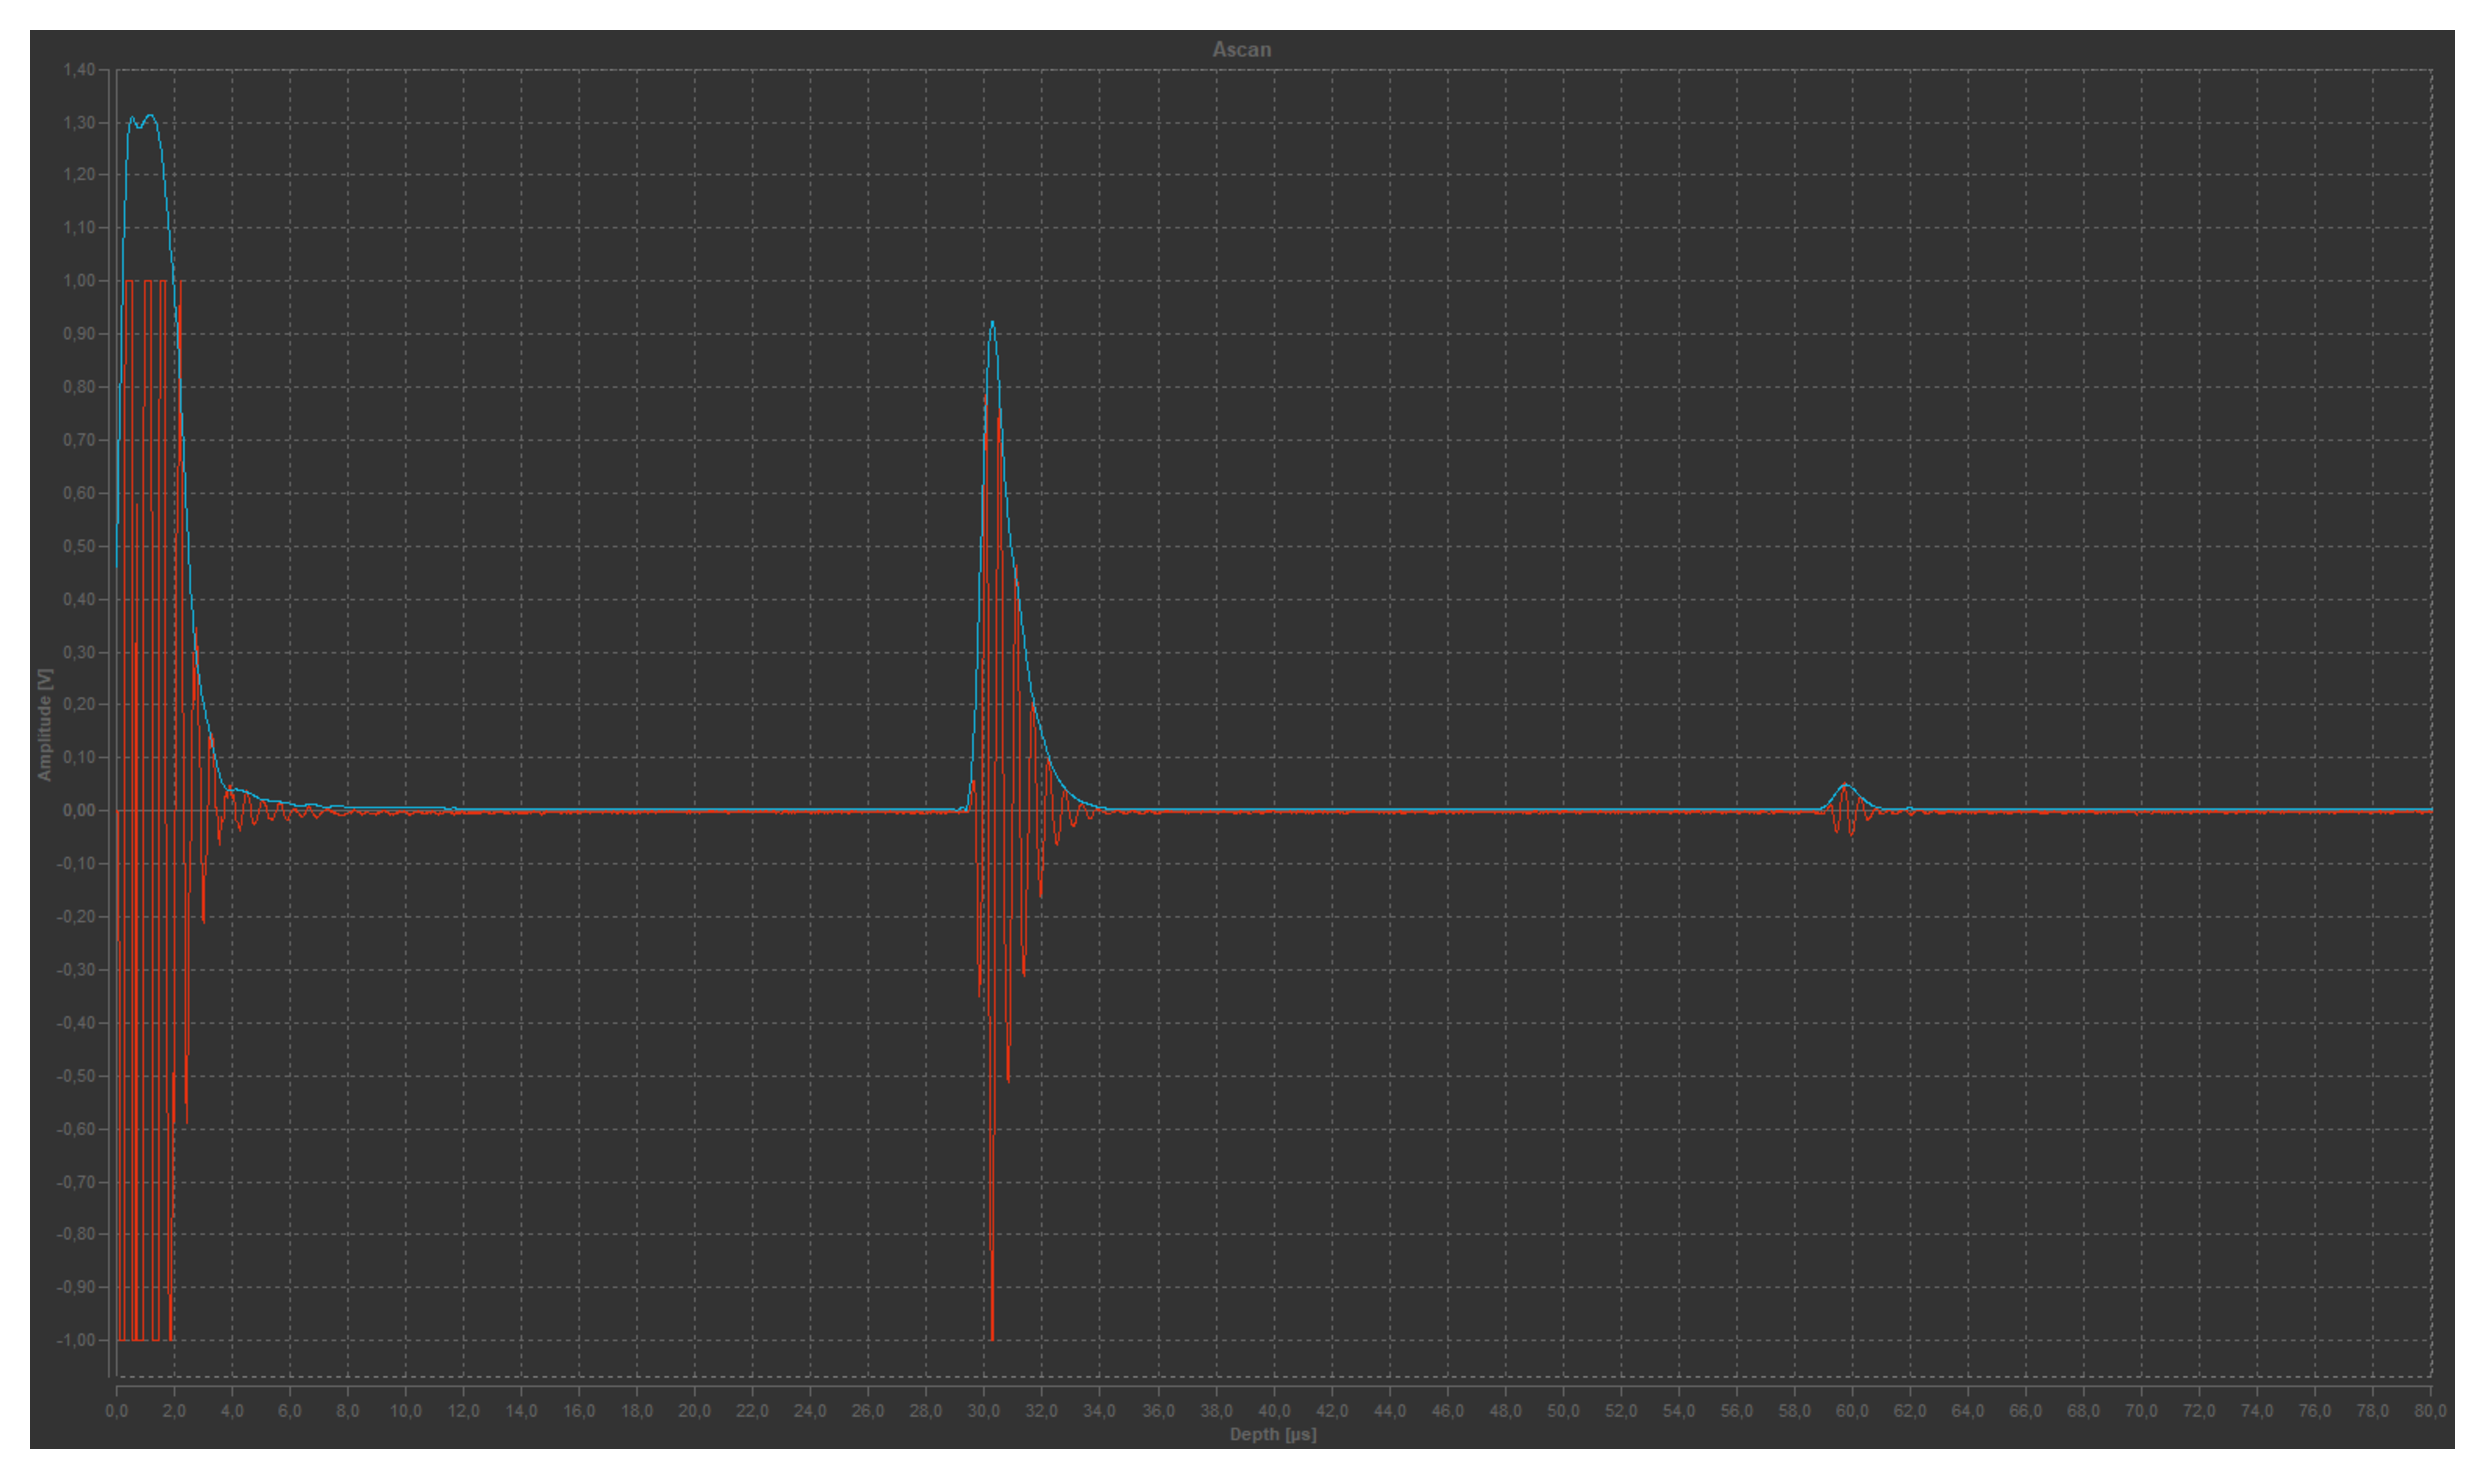
\includegraphics[width=\linewidth]{pictures/Impuls-Echo-Zylinder/z1.pdf}%
  \caption{Der erste Zylinder.}%
  \label{fig:echo_z1}%
  \end{subfigure}%
  \hfill%
  \begin{subfigure}{0.48\textwidth}%
  \centering%
  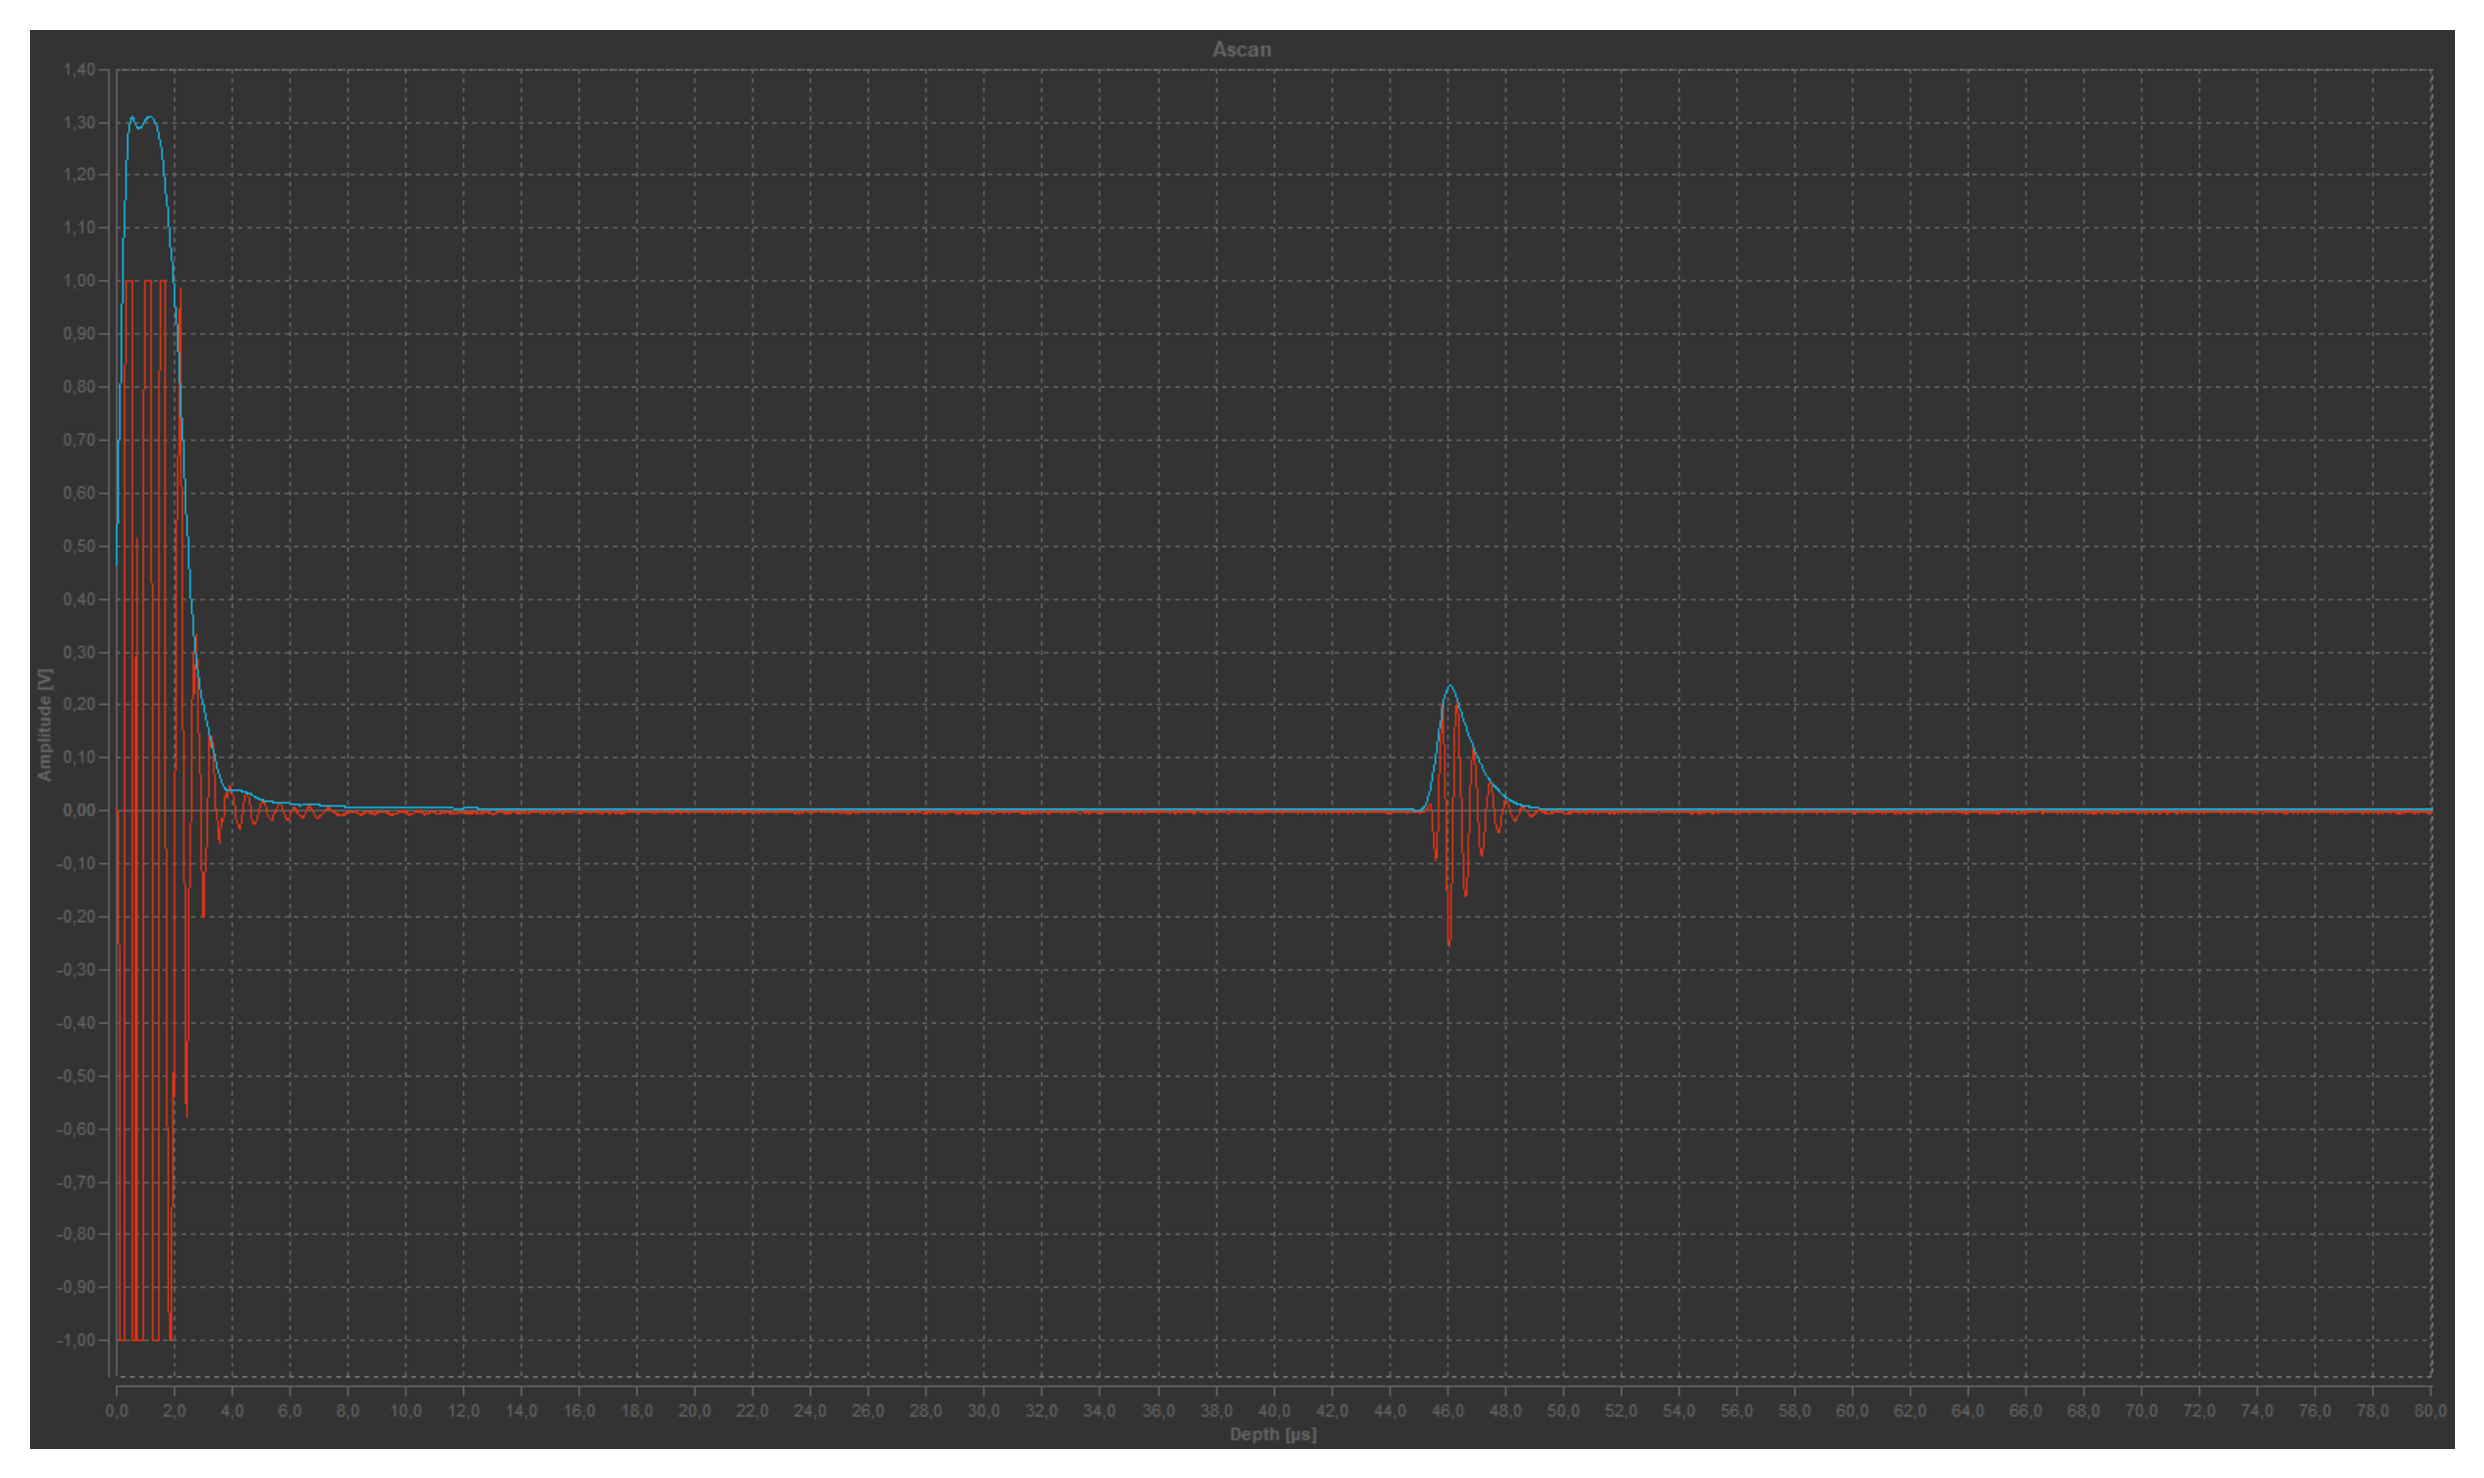
\includegraphics[width=\linewidth]{pictures/Impuls-Echo-Zylinder/z2.pdf}%
  \caption{Der zweite Zylinder.}%
  \label{fig:echo_z2}%
  \end{subfigure}%
  \hfill

  \begin{subfigure}{0.48\textwidth}%
  \centering%
  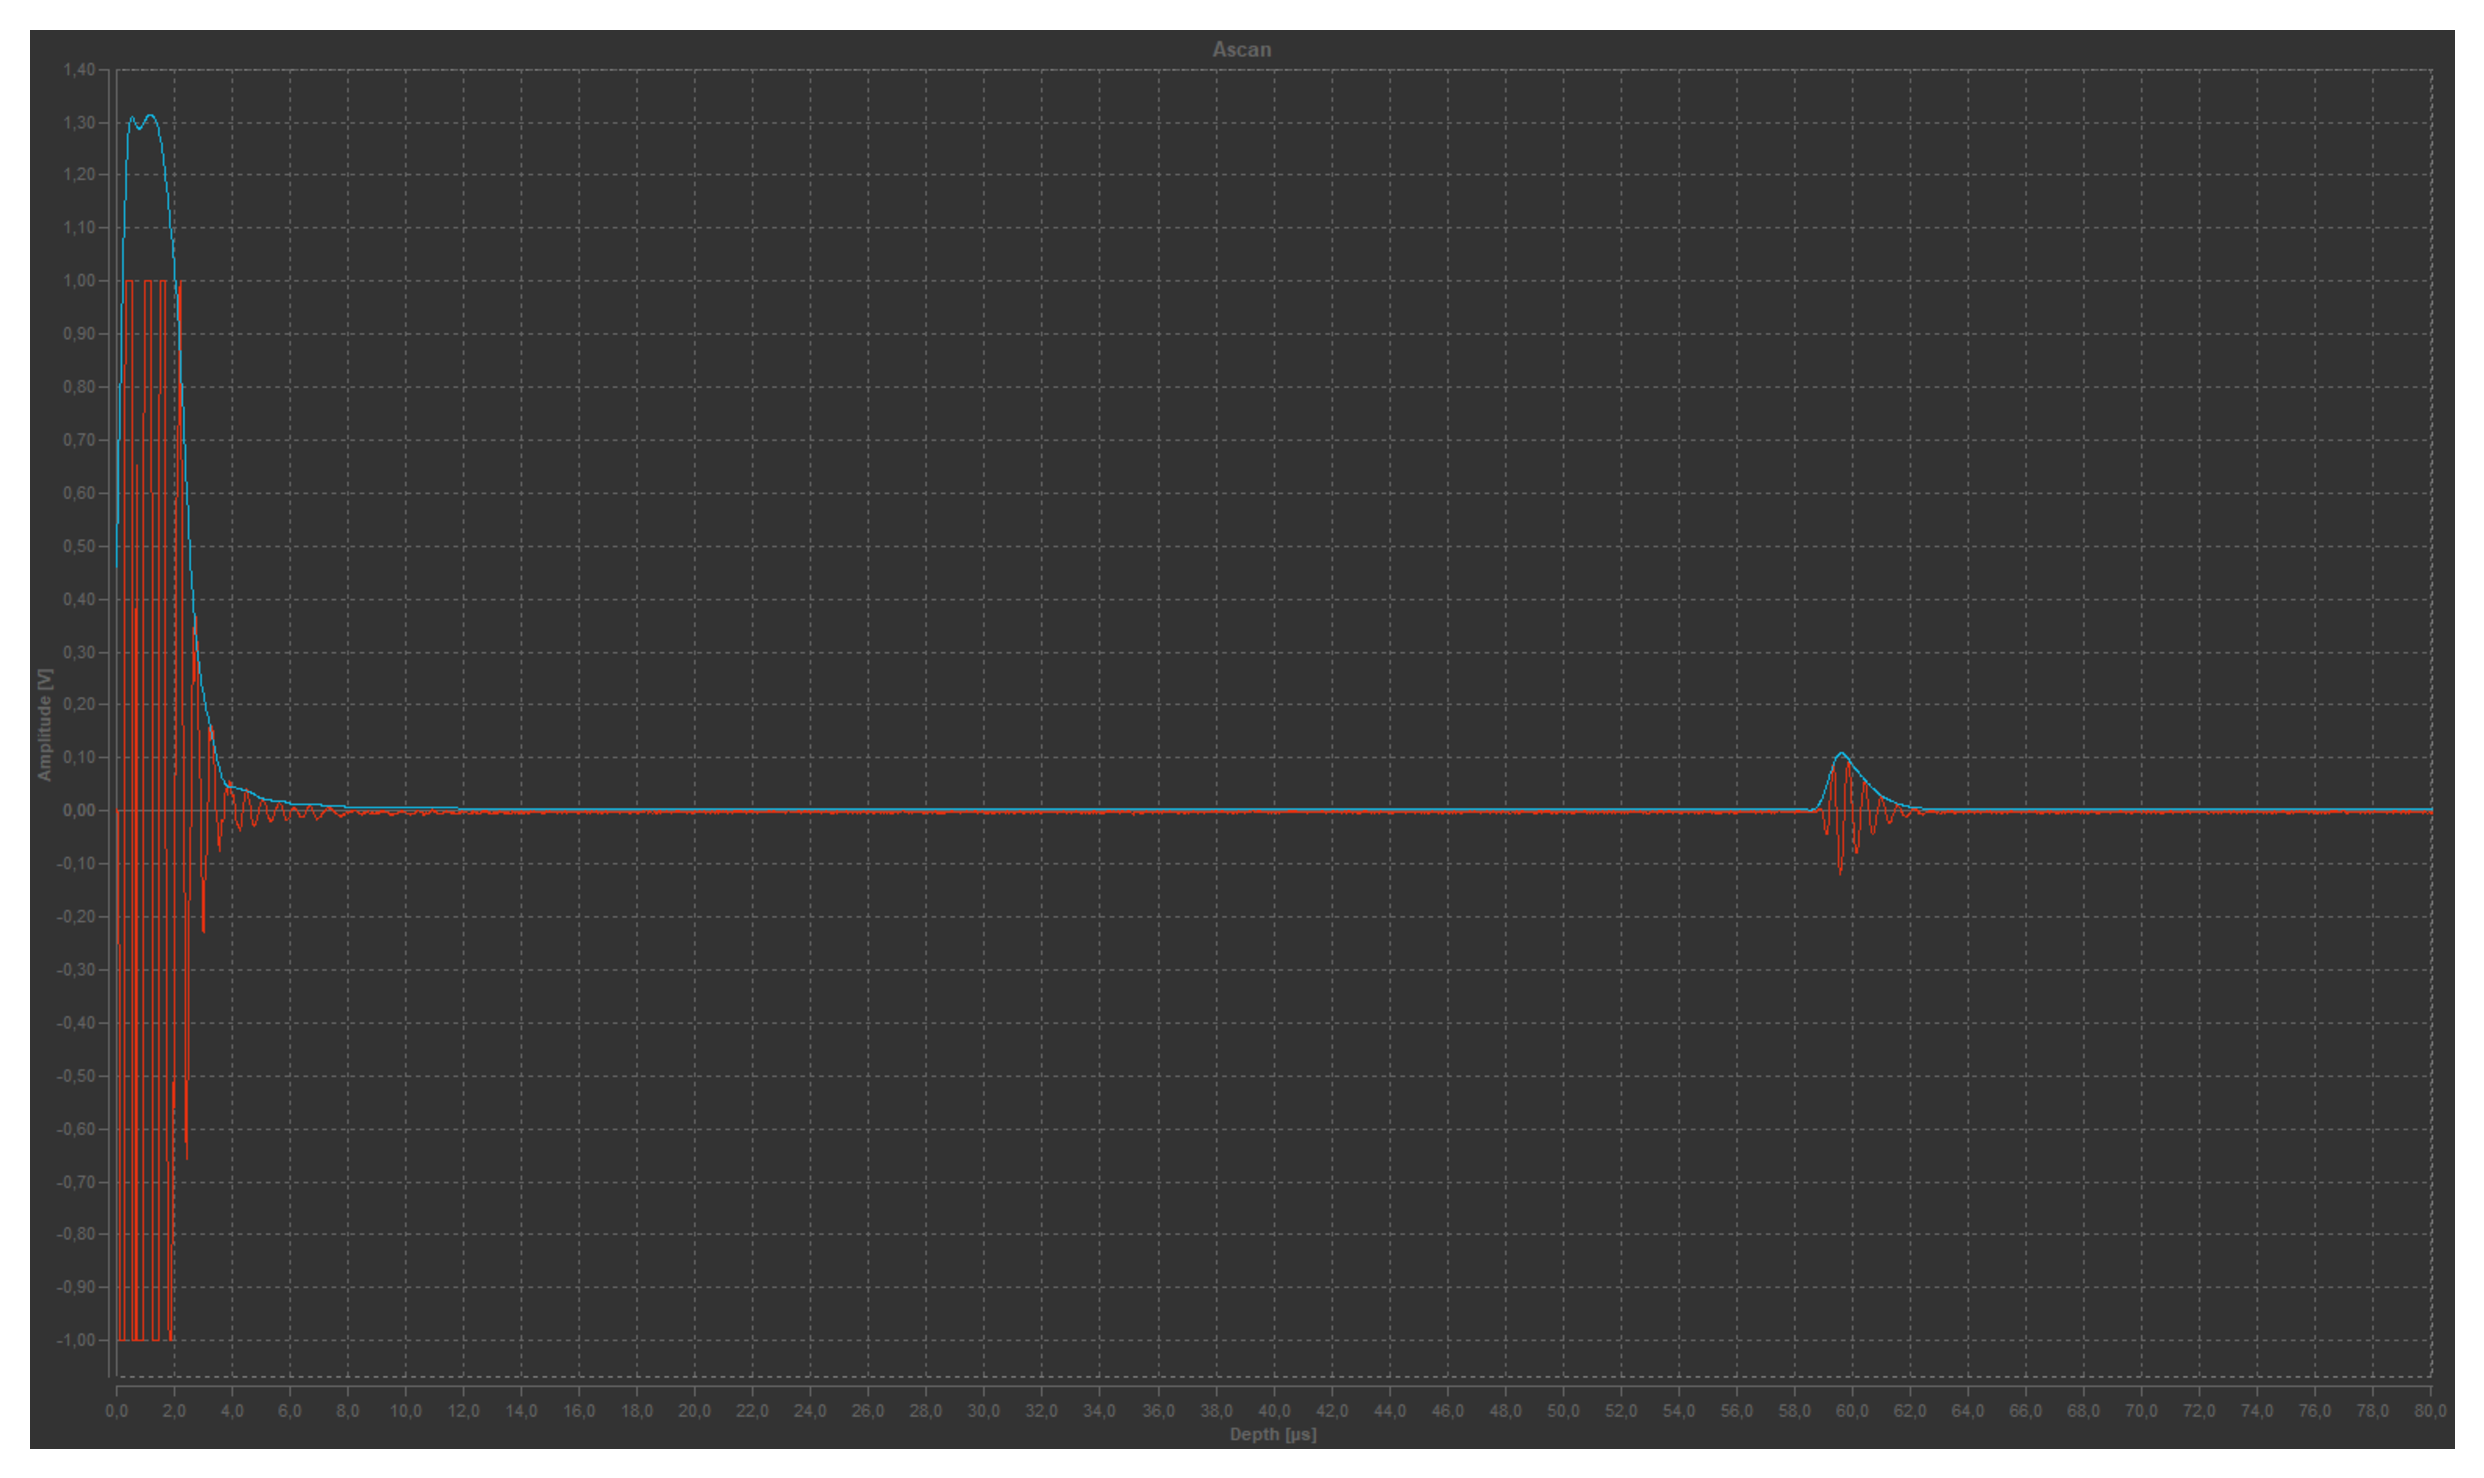
\includegraphics[width=\linewidth]{pictures/Impuls-Echo-Zylinder/z3.pdf}%
  \caption{Der dritte Zylinder.}%
  \label{fig:echo_z3}%
  \end{subfigure}%
  \hfill%
  \begin{subfigure}{0.48\textwidth}%
  \centering%
  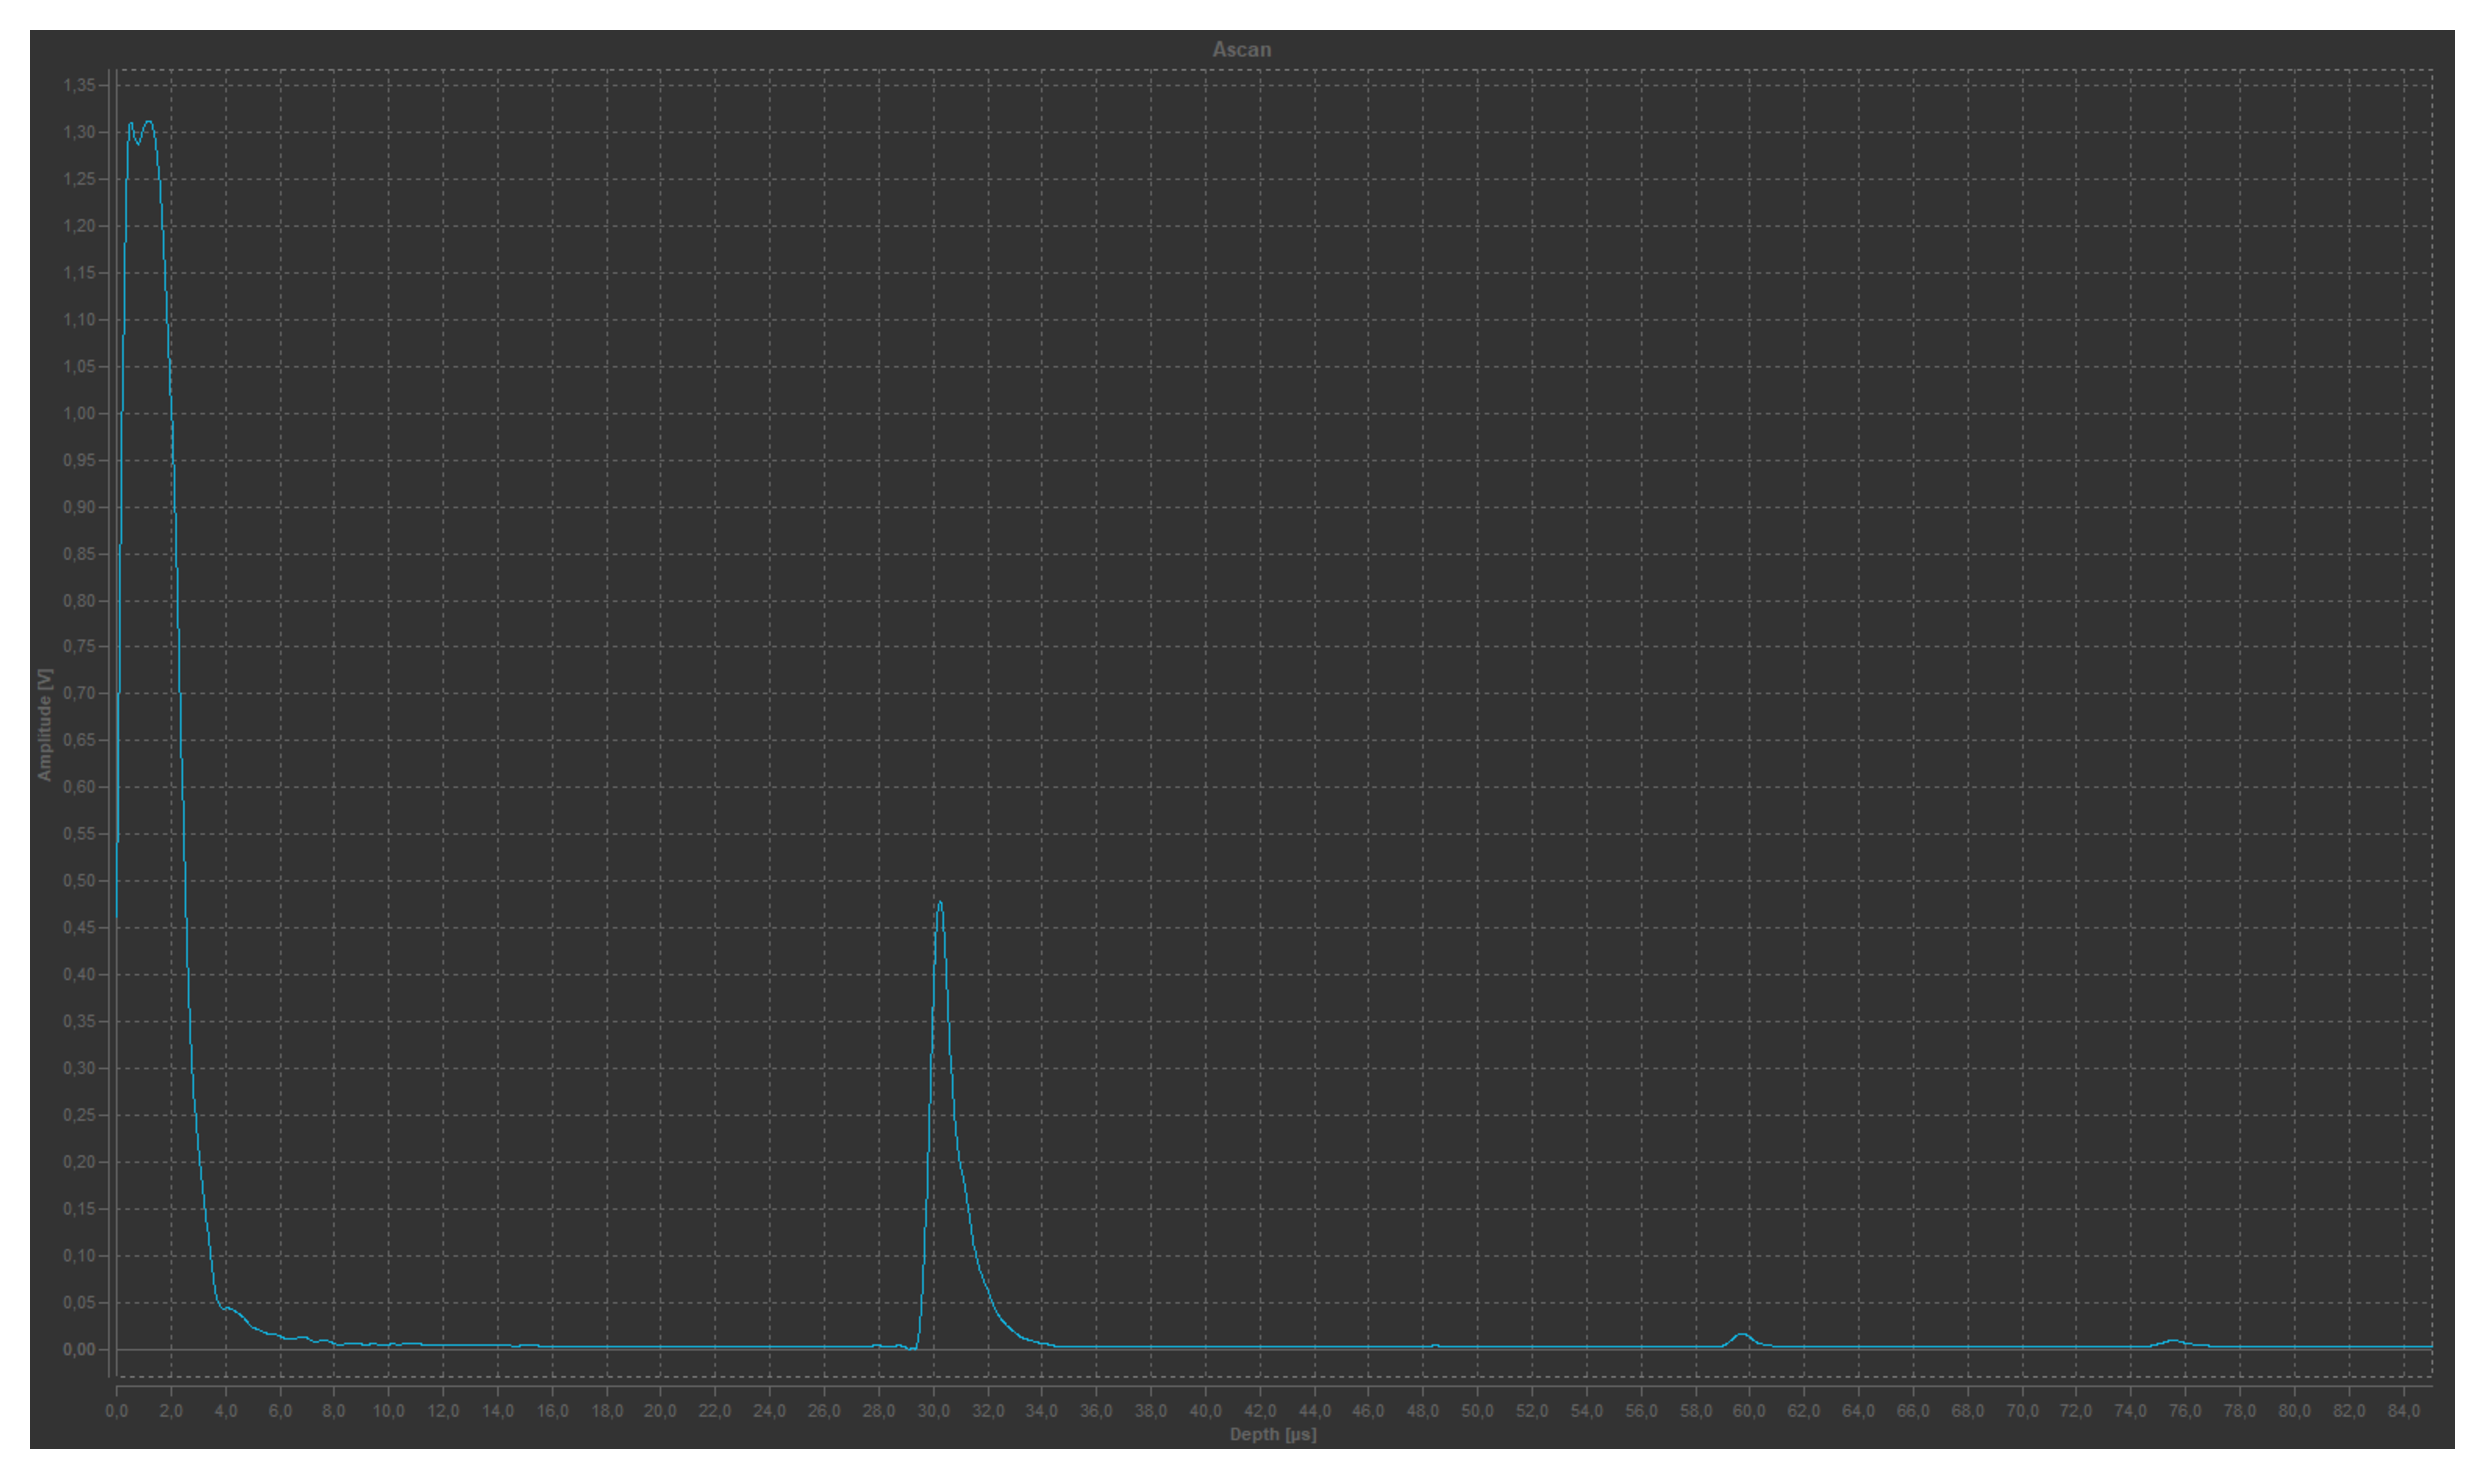
\includegraphics[width=\linewidth]{pictures/Impuls-Echo-Zylinder/z1_z2.pdf}%
  \caption{Der erste und zweite Zylinder zusammen.}%
  \label{fig:echo_z1_z2}%
  \end{subfigure}%
  \hfill

  \begin{subfigure}{0.48\textwidth}%
  \centering%
  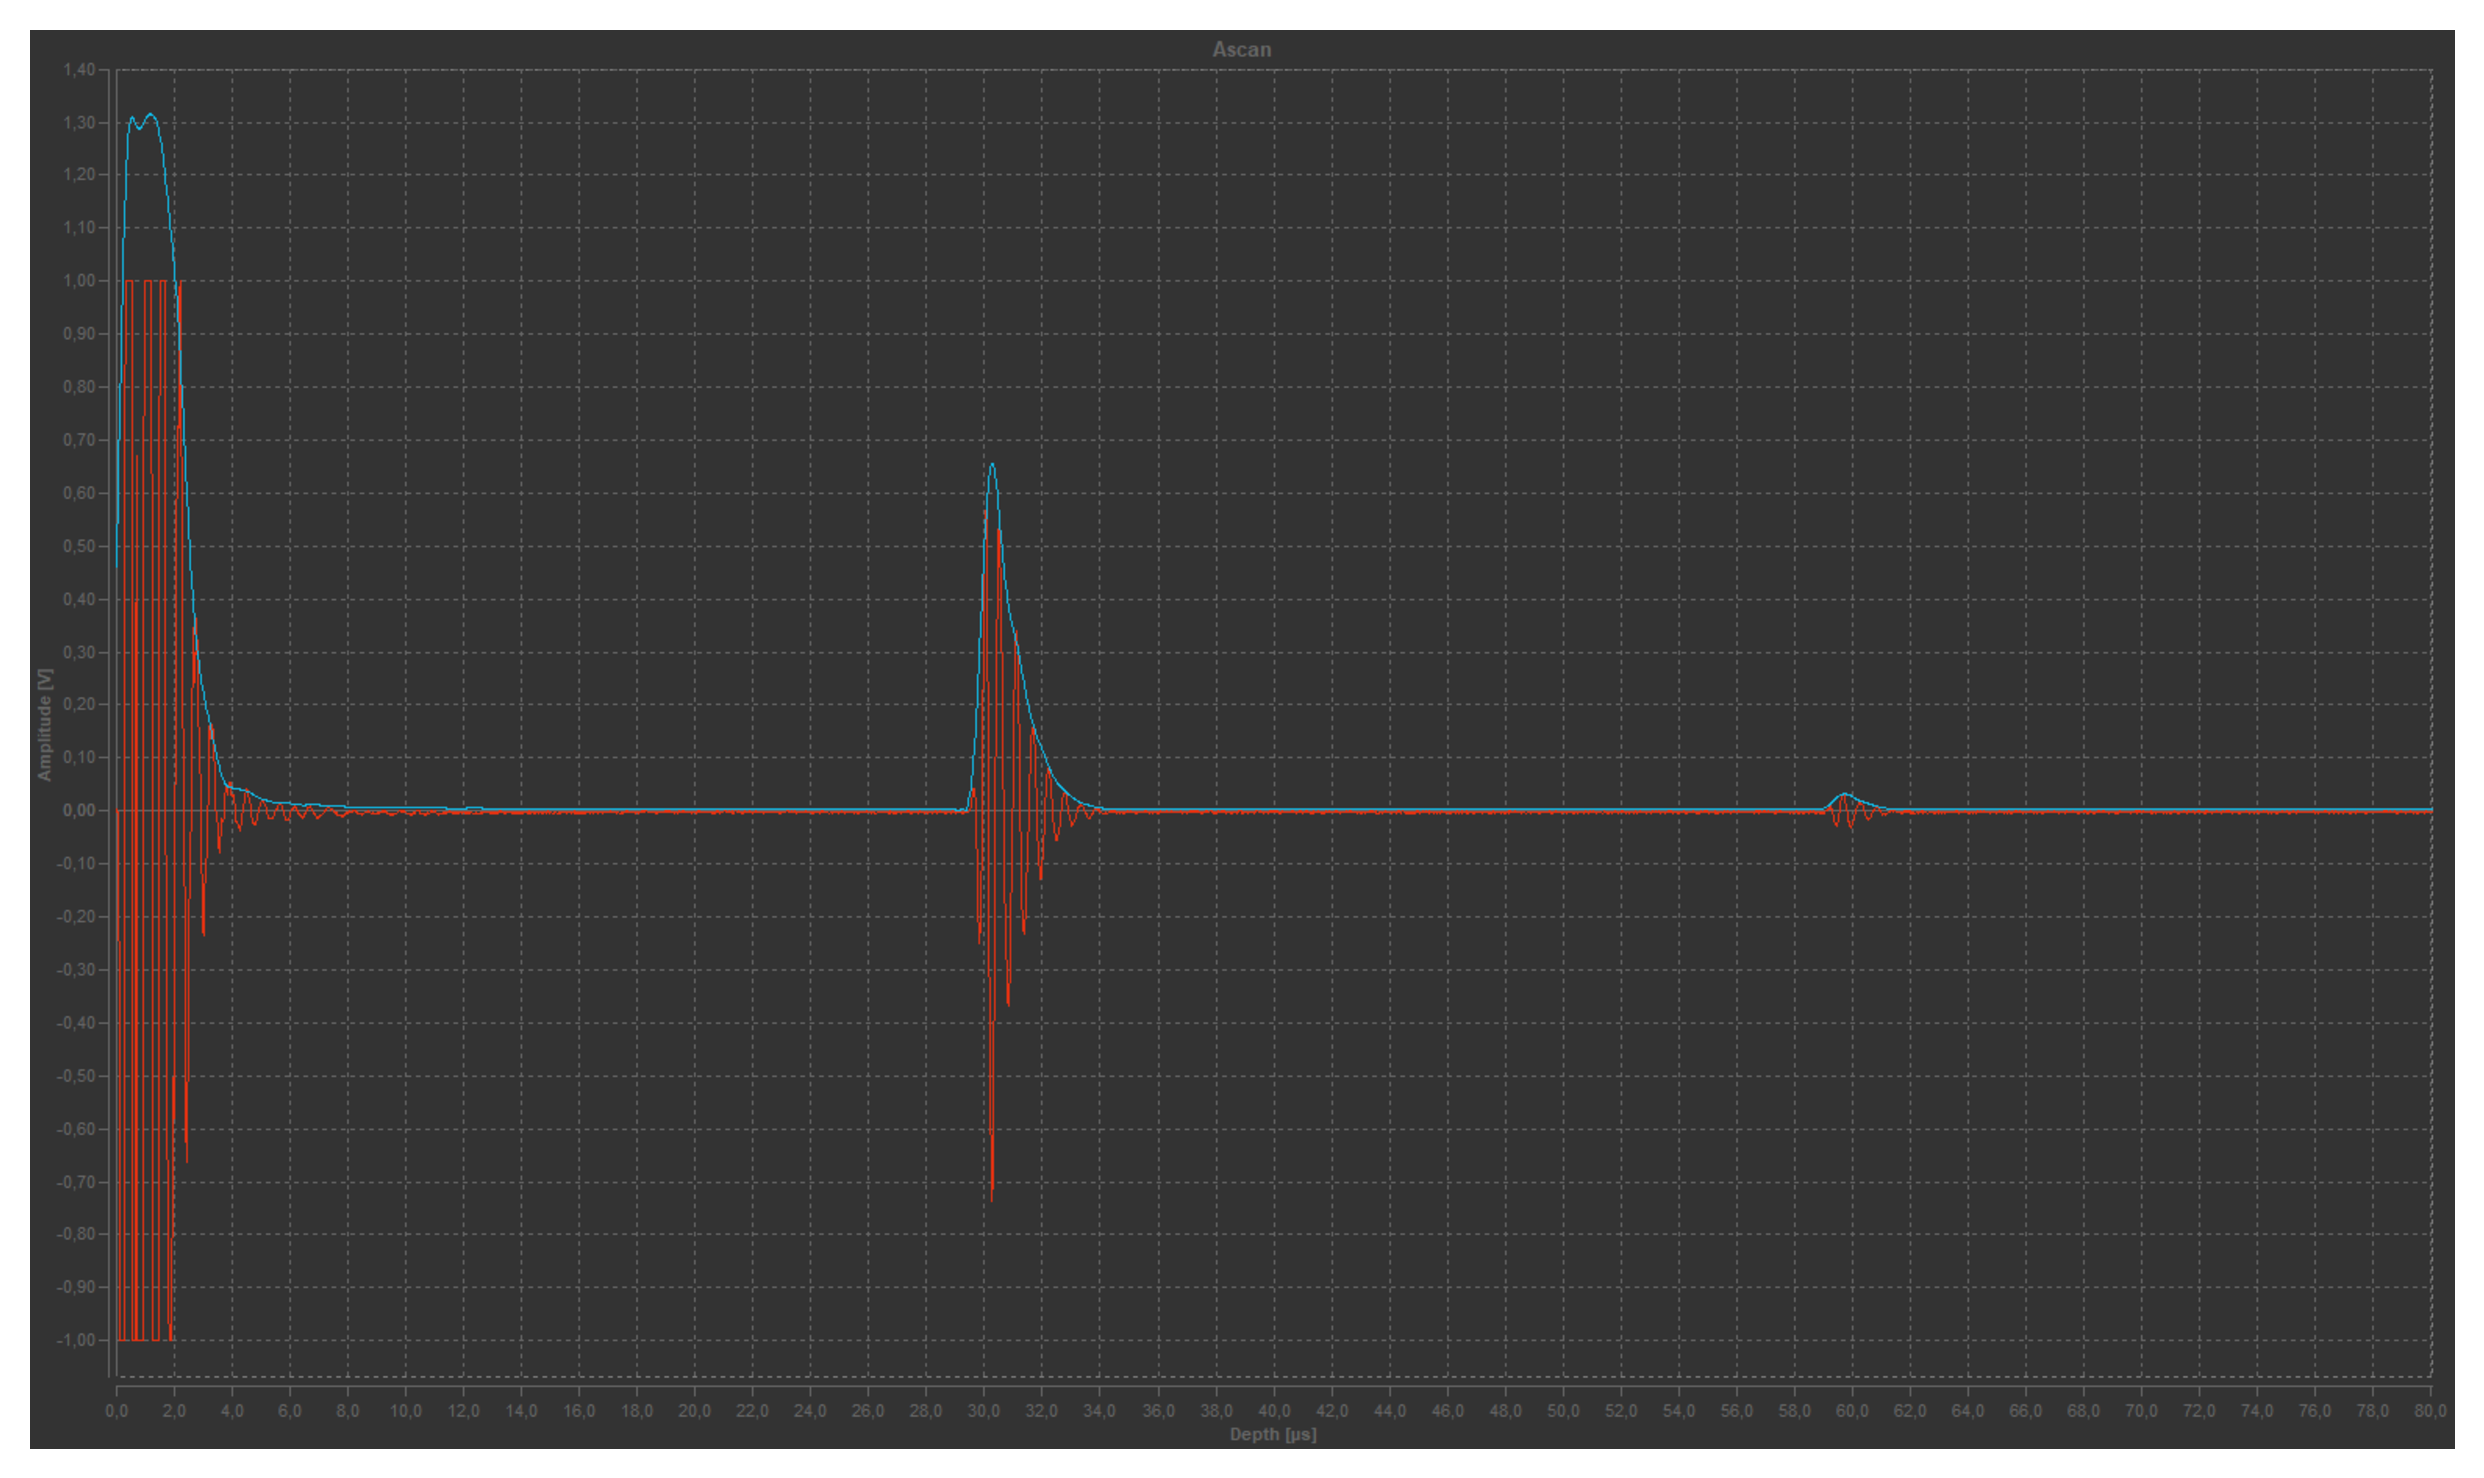
\includegraphics[width=\linewidth]{pictures/Impuls-Echo-Zylinder/z1_z3.pdf}%
  \caption{Der erste und der dritte Zylinder zusammen.}%
  \label{fig:echo_z1_z3}%
  \end{subfigure}%
  \hfill%
  \begin{subfigure}{0.48\textwidth}%
  \centering%
  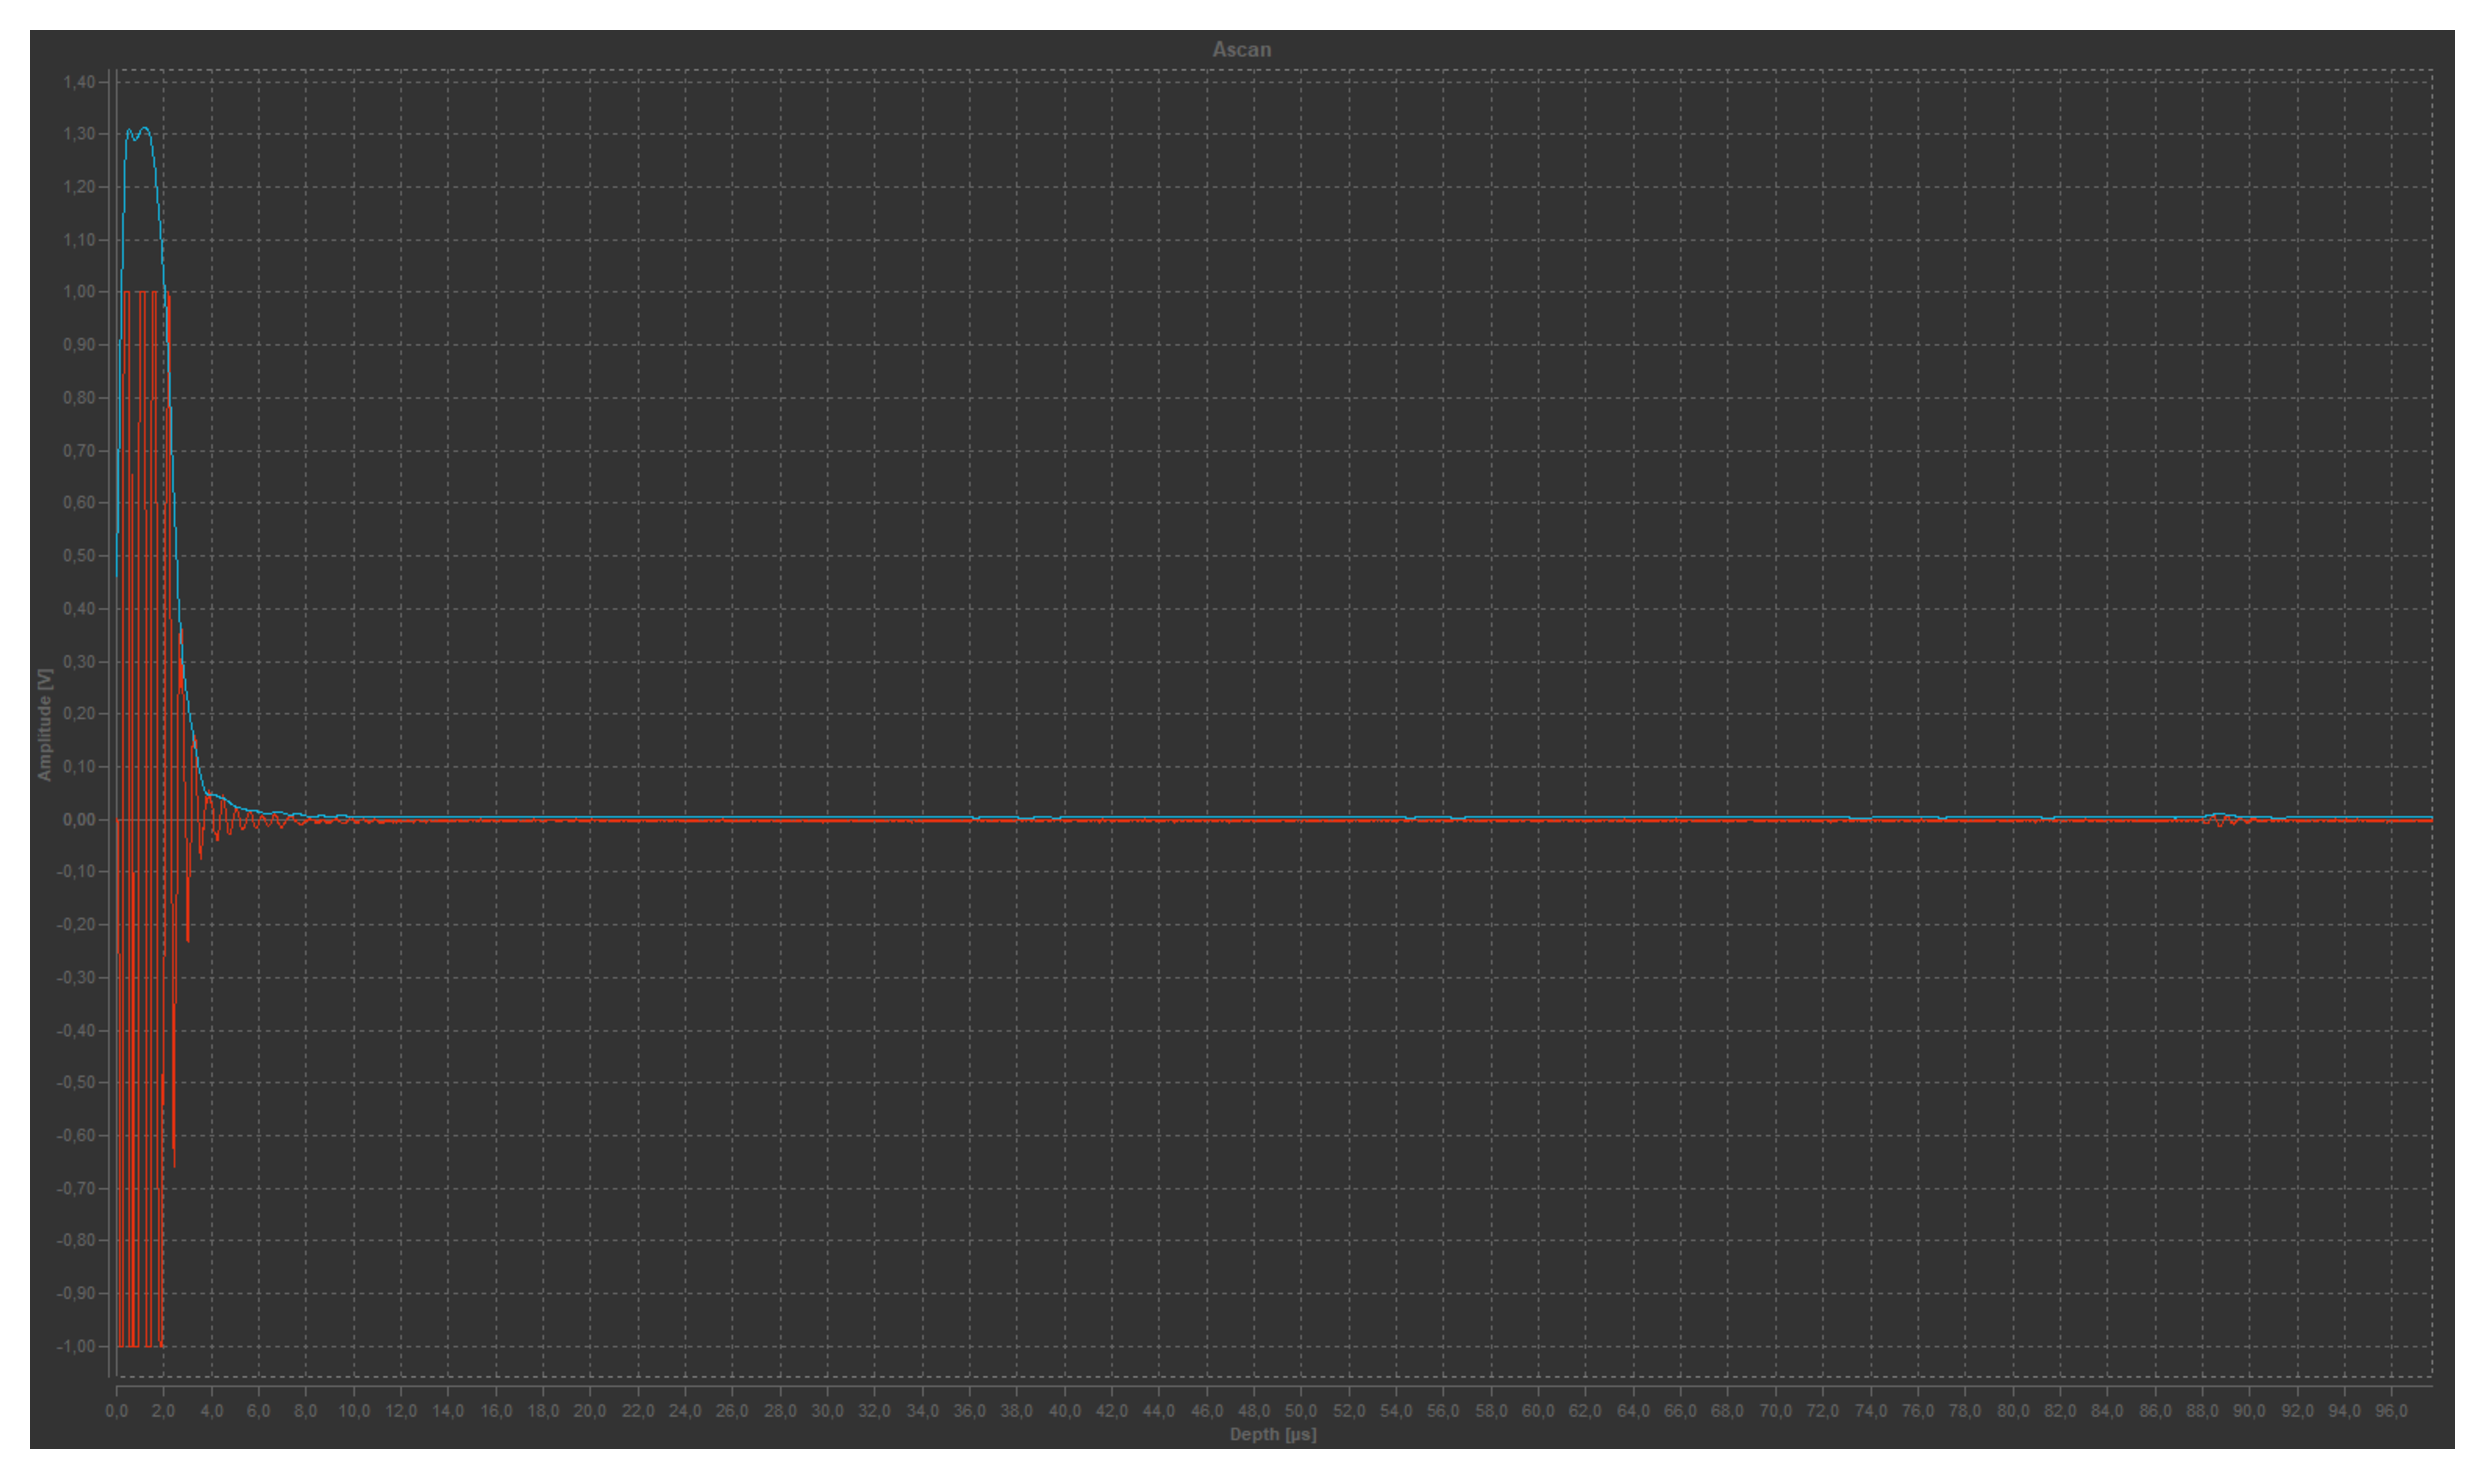
\includegraphics[width=\linewidth]{pictures/Impuls-Echo-Zylinder/z4_(1).pdf}%
  \caption{Der vierte Zylinder.}%
  \label{fig:echo_z4_(1)}%
  \end{subfigure}%
  \hfill

  \begin{subfigure}{\textwidth}%
  \centering%
  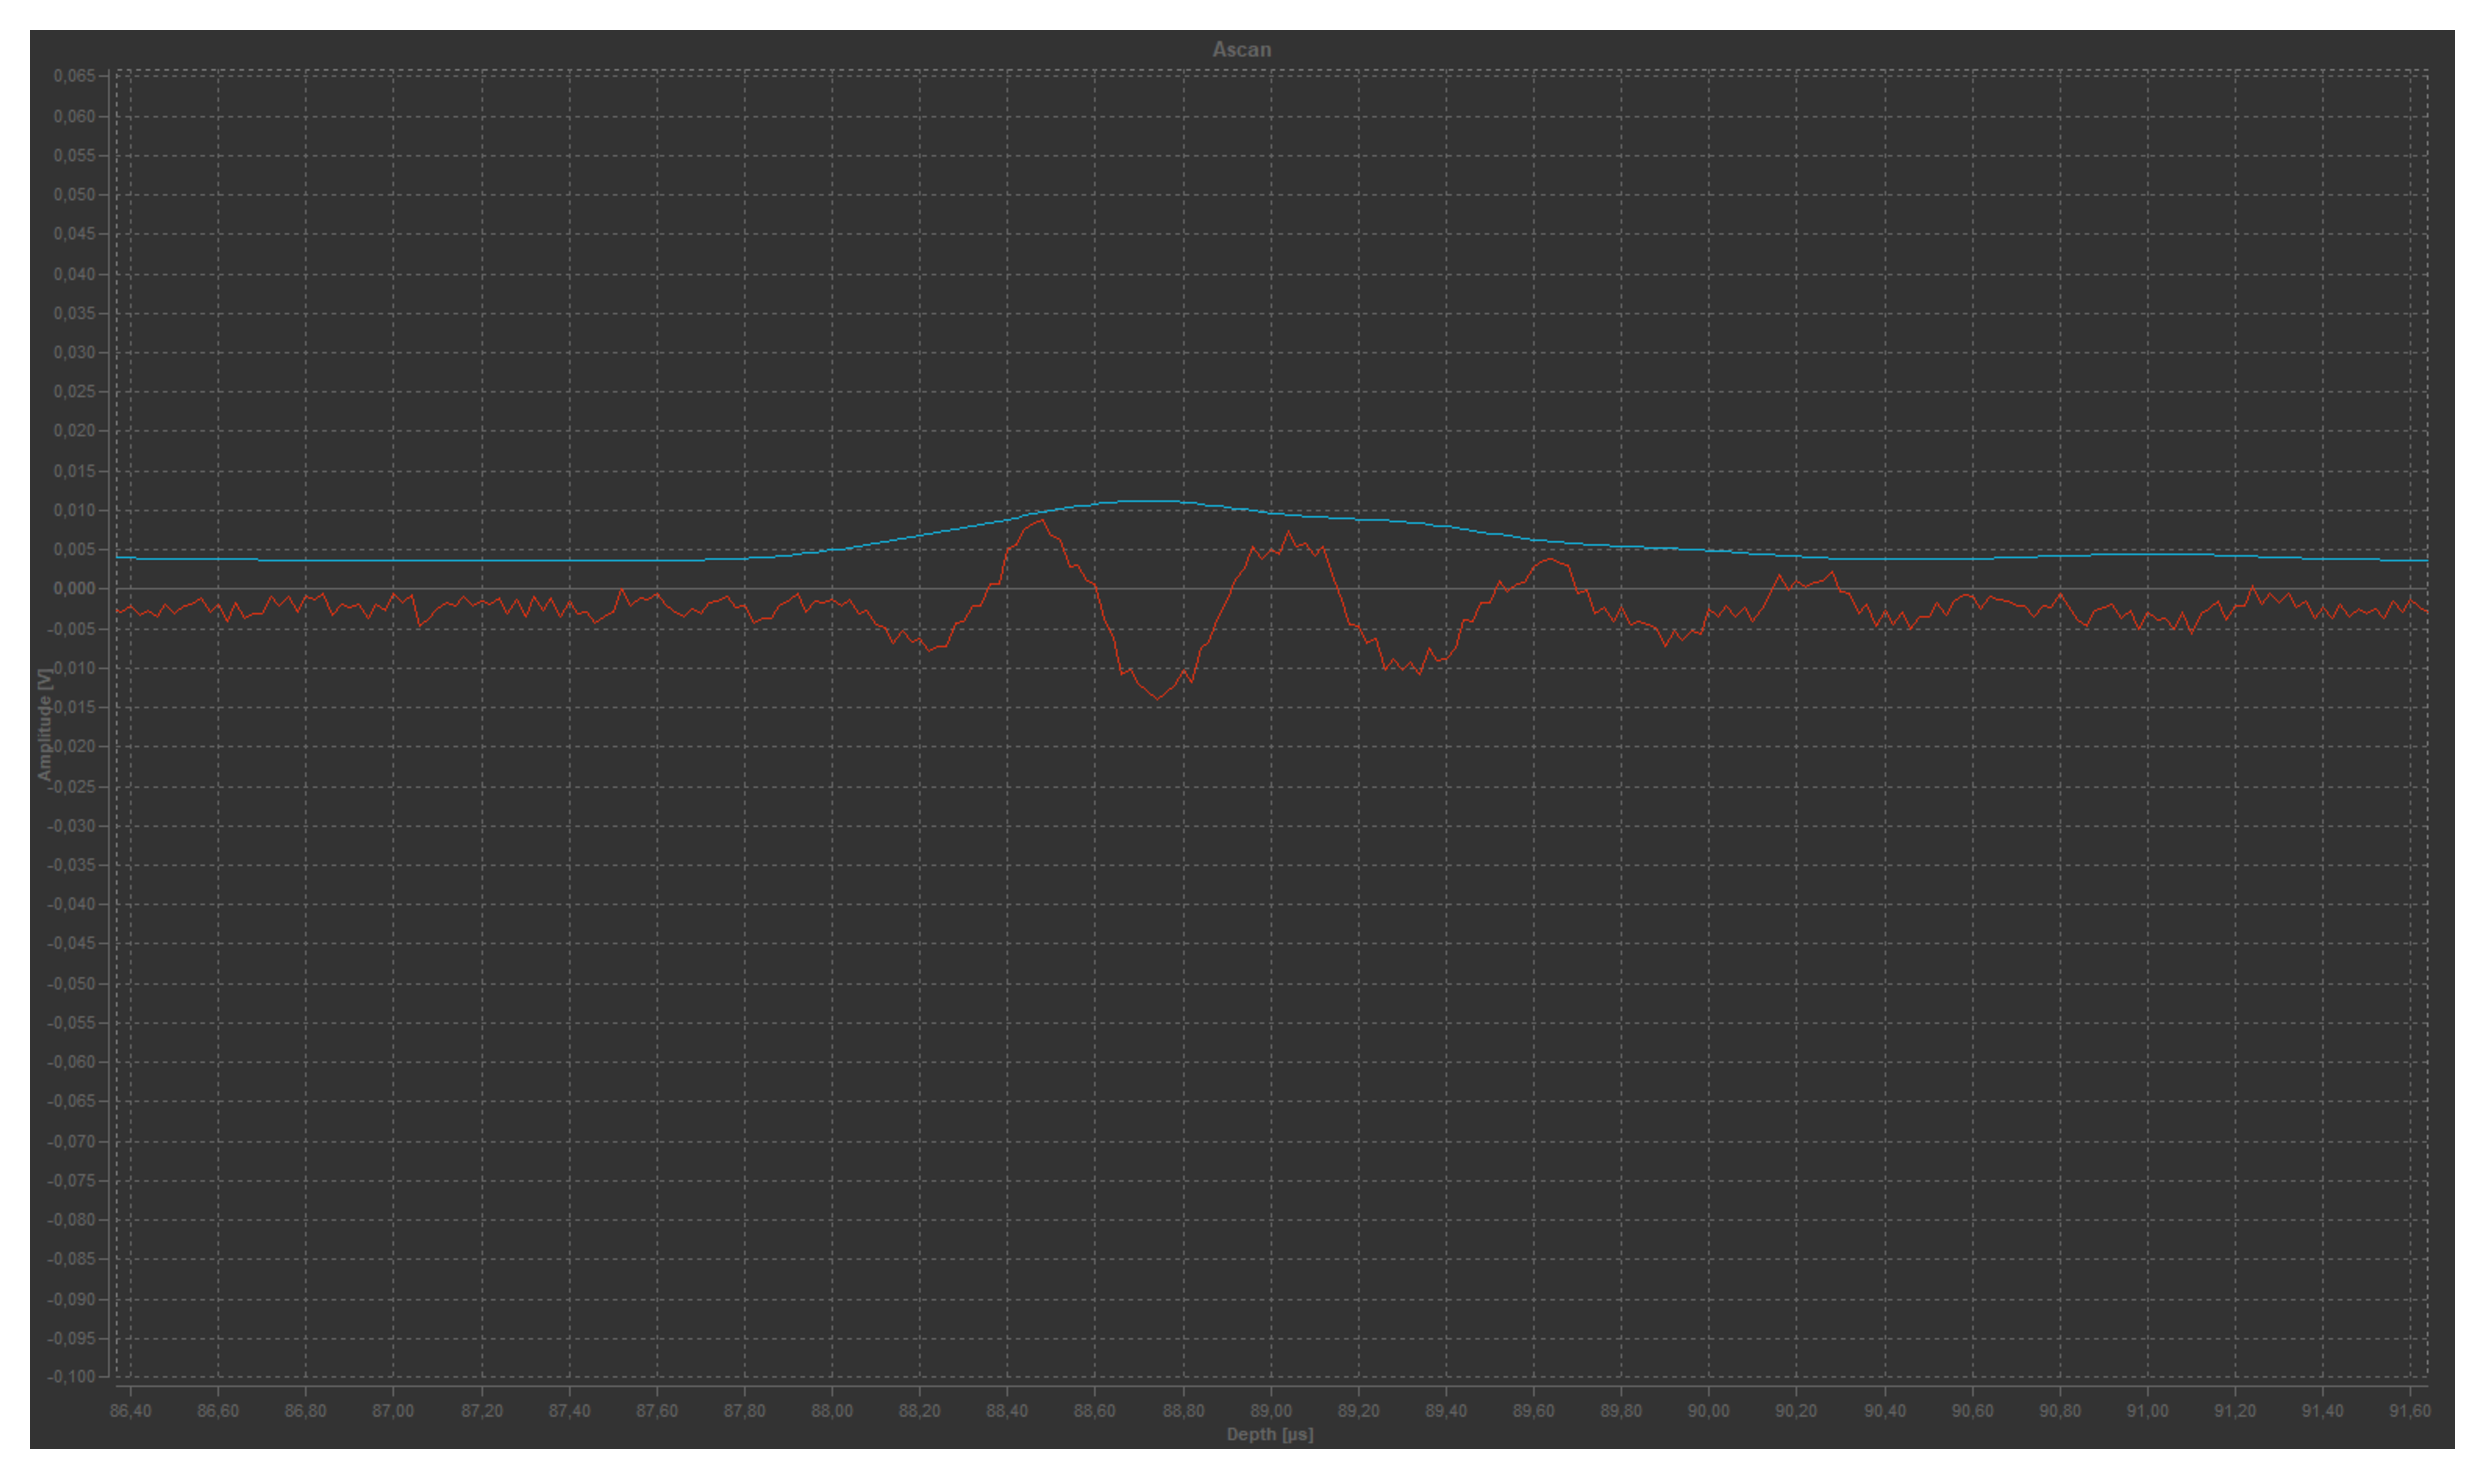
\includegraphics[width=0.48 \linewidth]{pictures/Impuls-Echo-Zylinder/z4_(2).pdf}%
  \caption{Der zweite Peak des vierten Zylinders in naher Aufnahme.}%
  \label{fig:echo_z4_(2)}%
  \end{subfigure}%
  \caption{Die Messungen des Impuls-Echo-Verfahrens}%
  \label{fig:echo_messungen}%
\end{figure}%


\subsection{Untersuchung des Augenmodells}

Die entsprechende Messung zu der Vermessung des Augenmodells ist in \autoref{fig:auge} dargestellt
und es sind fünf Peaks zu erkennen. Dabei ist der erste Peak (Peak 0) zu vernachlässigen.
Aus der Messung lassen sich dann die Messdaten in \autoref{tab:auge} ablesen.
Dabei werden die Peaks den folgenden Bestandteilen des Auges zugeordnet:
\begin{align*}
  \text{Peak 0} &\to \text{Hornhaut} \\
  \text{Peak 1} &\to \text{Anfang der Linse} \\
  \text{Peak 2} &\to \text{Ende der Linse} \\
  \text{Peak 3} &\to \text{Netzhaut} \\
  \text{Peak 4} &\to \text{Retina} \\  
\end{align*}
Mit den Schallgeschwindigkeiten $c_L = 2500 \unit{\meter / \second}$ und $c_{GK} = 1410 \unit{\meter / \second}$.
Aus der allgemeinen Formel \ref{tbd} ergeben sich dann
\begin{align*}
  \text{Hornhaut bis Anfang der Linse}&: s_1 = \frac{1}{2} c_{GK} \cdot t_1 = 0.846 \, \unit{\centi\meter} \\
  \text{Hornhaut bis Ende der Linse}&: s_2 = \frac{1}{2} c_L \cdot (t_2 - t_1) + s_1 = 1.346 \, \unit{\centi\meter} \\
  \text{Hornhaut bis Netzhaut}&: s_3 = \frac{1}{2} c_{GK} \cdot (t_3 - t_2) + s_2 = 1.834 \, \unit{\centi\meter} \\
  \text{Hornhaut bis Retina}&: s_4 = \frac{1}{2} c_{L} \cdot (t_4 - t_3) + s_3 = 8.59 \, \unit{\centi\meter} 
\end{align*}


\begin{table}
  \centering
  \caption{Messdaten der Vermessung des Auges.}
  \label{tab:auge}
  \begin{tabular}{c c}
      \toprule
      Peak Nummer & t / \unit{\micro\second}\\ 
      \midrule
      1 & 12\\
      2 & 16\\
      3 & 23\\
      4 & 77\\
      \bottomrule
  \end{tabular}
\end{table}

\begin{figure}
  \centering
  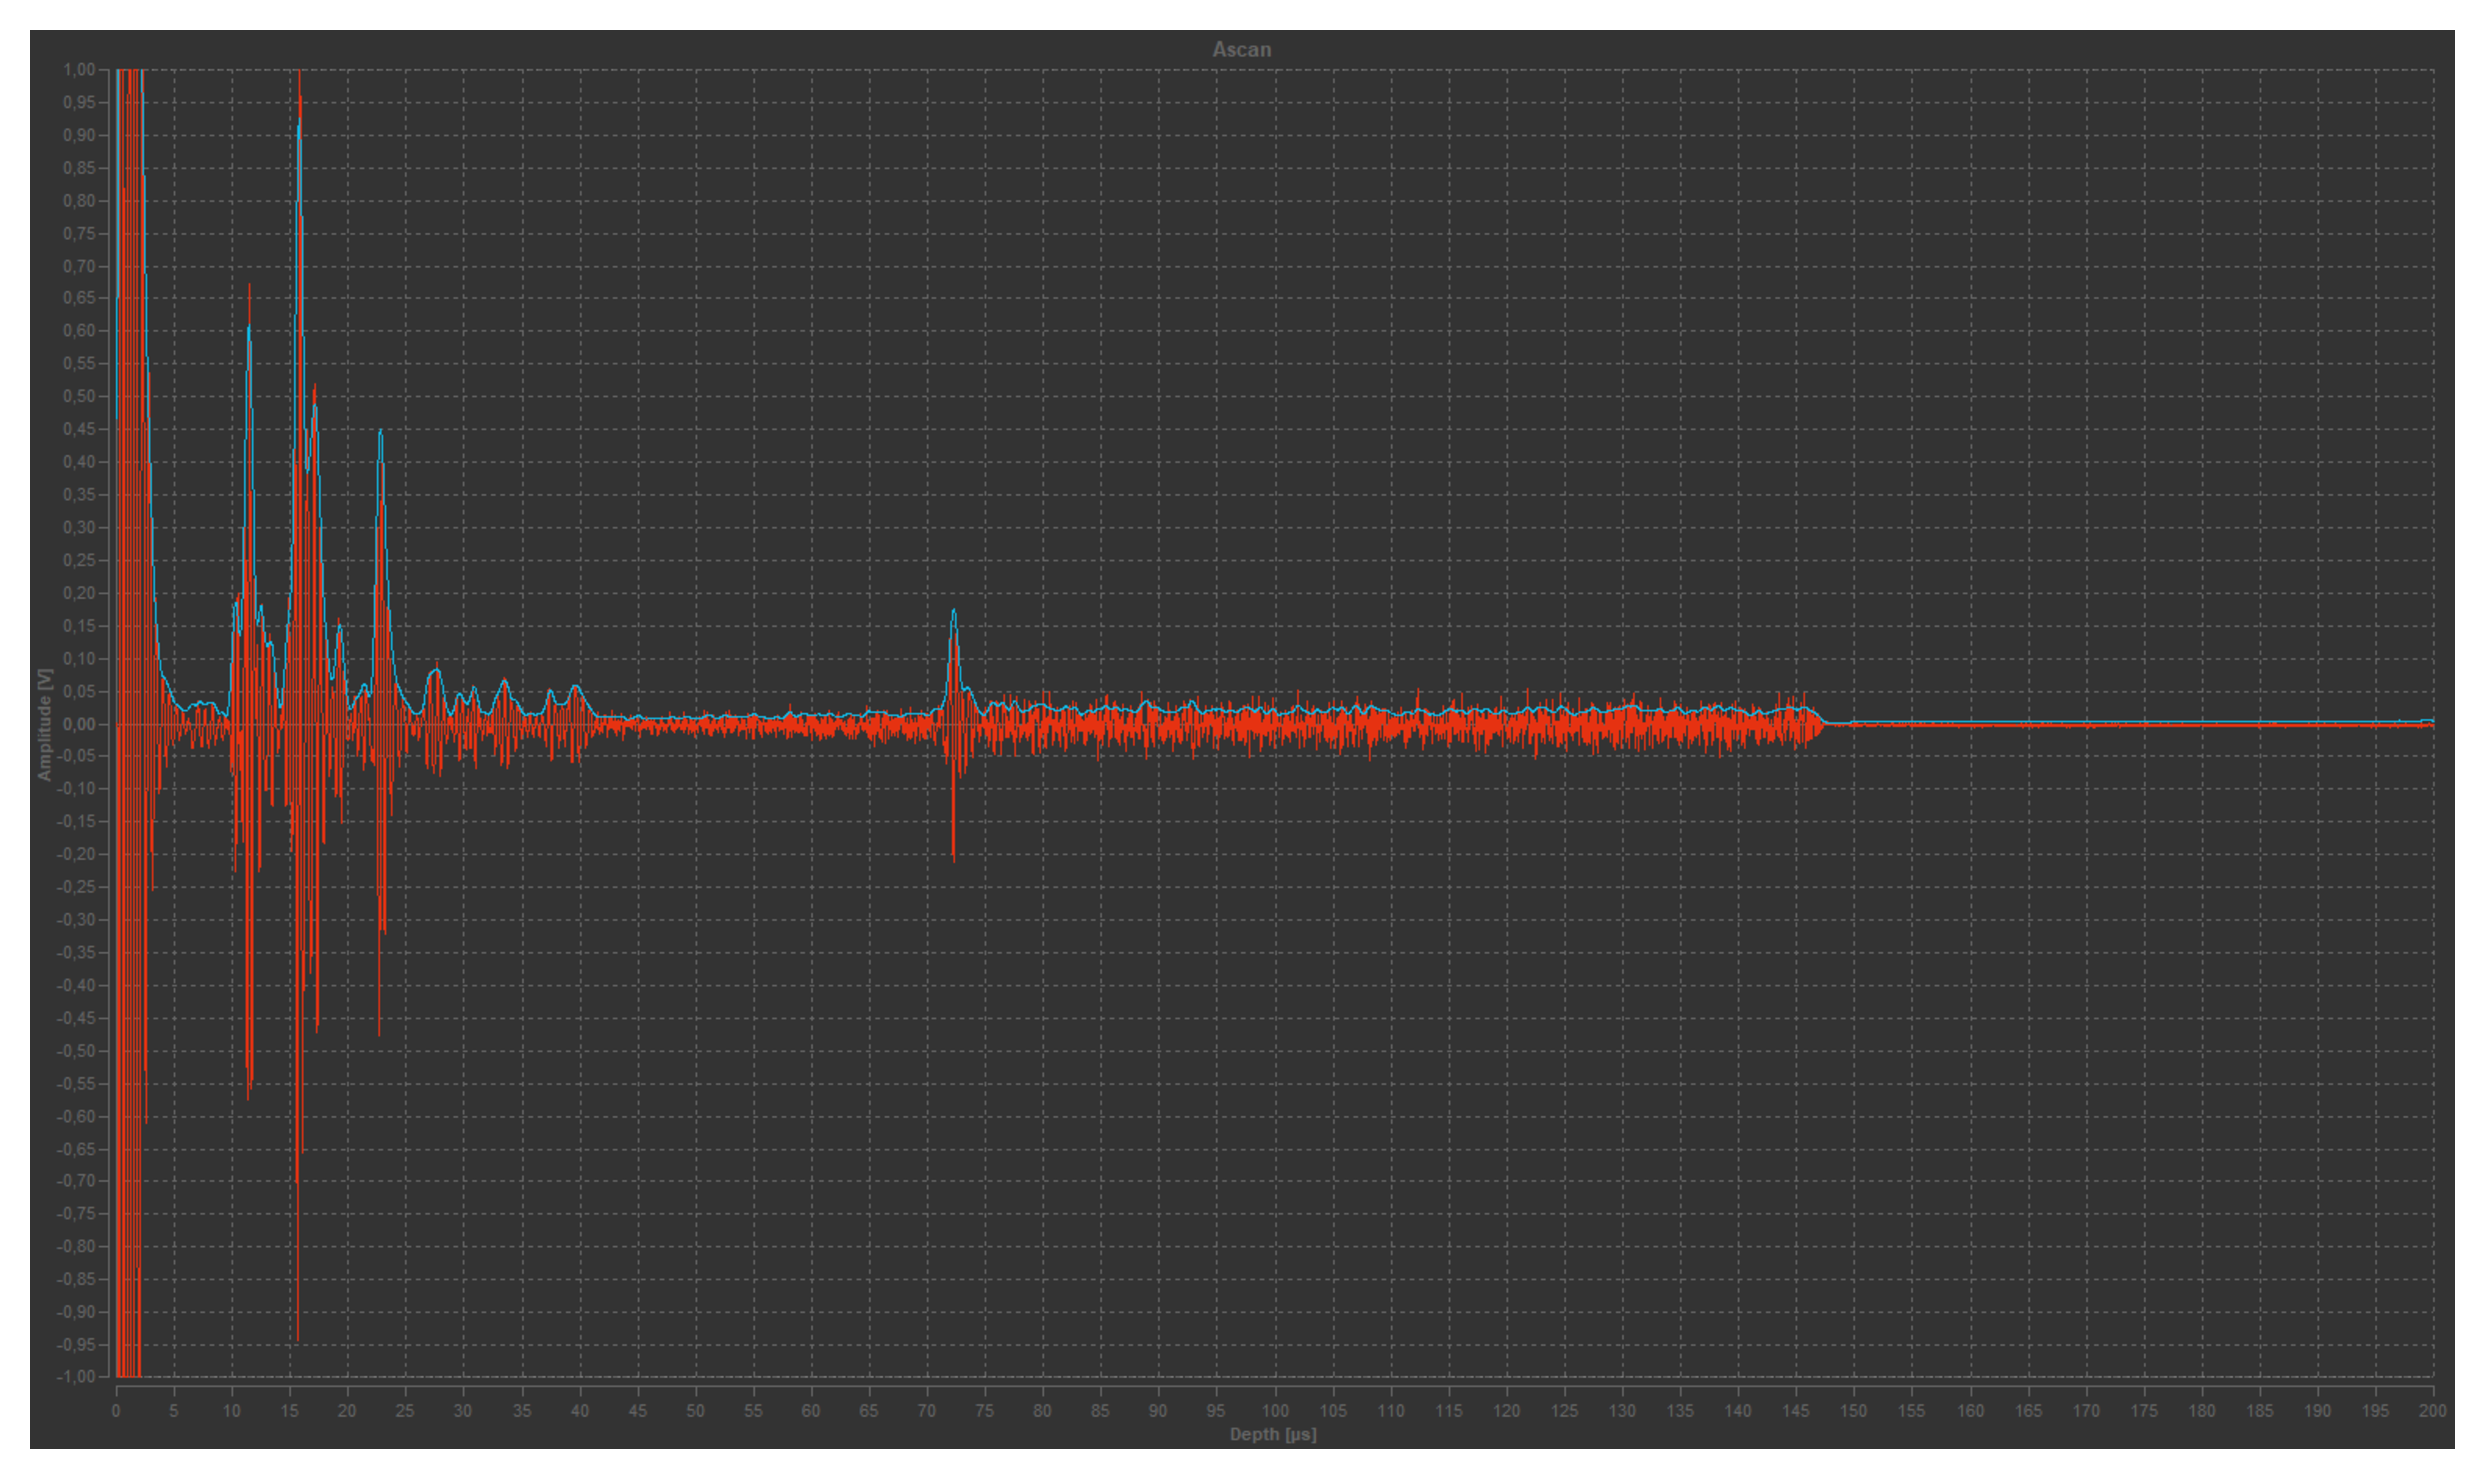
\includegraphics[width = 0.8\linewidth]{pictures/auge/Messung1Auge.pdf}
  \caption{Screenshot der Messung des Augenmodells}
  \label{fig:auge}
\end{figure}